
          %--------------------%
\chapter{~~Meshes and manifolds; patchwork}\label{\numb section 2}
          %--------------------%

This section describes several examples of meshes, some of them built on specific manifolds.
Note that in this manual we use the term ``manifold'' to mean a manifold without boundary.

This section focuses on building meshes by joining together several regular meshes
(triangles or quadrangles), like patches.
In contrast, section \ref{\numb section 3} shows how to mesh regions of a manifold
by progressively adding triangular cells, one by one.

Paragraphs \ref{\numb section 2.\numb parag 4}, \ref{\numb section 2.\numb parag 5},
\ref{\numb section 2.\numb parag 9} and \ref{\numb section 2.\numb parag 10} deal
with one-dimensional meshes (curves) in $ \mathbb{R}^2 $,
paragraphs \ref{\numb section 2.\numb parag 12}, \ref{\numb section 2.\numb parag 13},
\ref{\numb section 2.\numb parag 14} and \ref{\numb section 2.\numb parag 15} show
curves in $ \mathbb{R}^3 $,
paragraphs \ref{\numb section 2.\numb parag 1}, \ref{\numb section 2.\numb parag 2},
\ref{\numb section 2.\numb parag 3}, \ref{\numb section 2.\numb parag 9} and
\ref{\numb section 2.\numb parag 10} show plane domains
(two-dimensional meshes in $ \mathbb{R}^2 $),
while paragraphs \ref{\numb section 2.\numb parag 6}, \ref{\numb section 2.\numb parag 7},
\ref{\numb section 2.\numb parag 8}, \ref{\numb section 2.\numb parag 12},
\ref{\numb section 2.\numb parag 13}, \ref{\numb section 2.\numb parag 16} and
\ref{\numb section 2.\numb parag 17} focus on two-dimensional meshes
in $ \mathbb{R}^3 $ (surfaces).

Paragraphs \ref{\numb section 2.\numb parag 4} -- \ref{\numb section 2.\numb parag 13}
are about manifolds defined implicitly as level sets;
paragraphs \ref{\numb section 2.\numb parag 14} -- \ref{\numb section 2.\numb parag 17}
describe parametric manifolds.


          %----------------%
\section{~~Joining segments}\label{\numb section 2.\numb parag 1}
          %----------------%

Here is another way of meshing the same L-shaped domain as in paragraph
\ref{\numb section 1.\numb parag 3} :

\begin{figure}[ht] \centering
  \psfrag{A}{\tt\textcolor{textindraw}{A}}
  \psfrag{B}{\tt\textcolor{textindraw}{B}}
  \psfrag{C}{\tt\textcolor{textindraw}{C}}
  \psfrag{D}{\tt\textcolor{textindraw}{D}}
  \psfrag{E}{\tt\textcolor{textindraw}{E}}
  \psfrag{F}{\tt\textcolor{textindraw}{F}}
  \psfrag{G}{\tt\textcolor{textindraw}{G}}
  \psfrag{H}{\tt\textcolor{textindraw}{H}}
  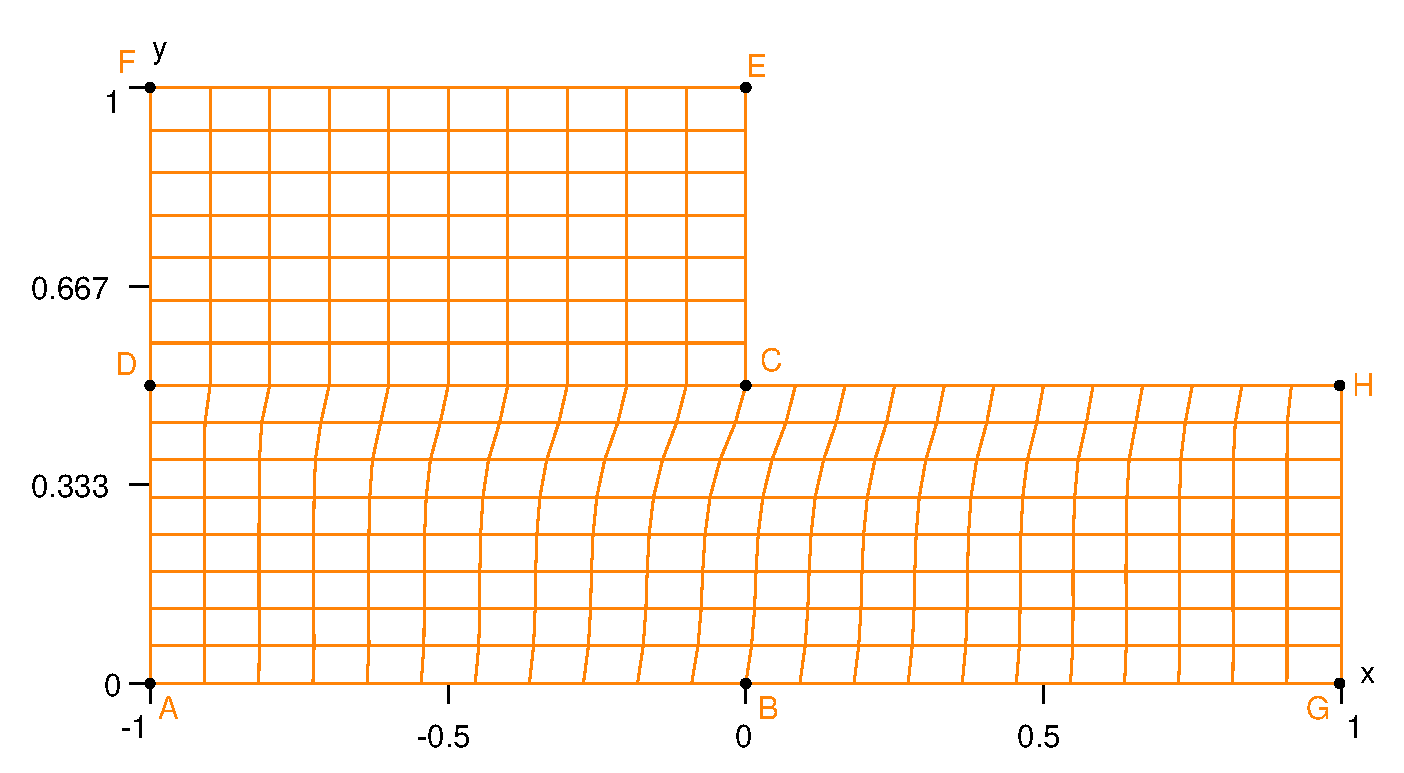
\includegraphics[width=95mm]{L-shaped-distorted}
  \caption{An L-shaped mesh again}
  \label{\numb section 2.\numb fig 1}
\end{figure}

\begin{Verbatim}[commandchars=\\\{\},formatcom=\small\tt,frame=single,
   label=parag-\ref{\numb section 2.\numb parag 1}.cpp,rulecolor=\color{coment},
   baselinestretch=0.94,framesep=2mm]
   \verm{Mesh} \azul{AG} ( \verm{tag}::segment, A.reverse(), G, \verm{tag}::divided_in, 22 );
   \verm{Mesh} \azul{GH} ( \verm{tag}::segment, G.reverse(), H, \verm{tag}::divided_in, 8 );
   \verm{Mesh} \azul{HC} ( \verm{tag}::segment, H.reverse(), C, \verm{tag}::divided_in, 12 );
   \verm{Mesh} \azul{CD} ( \verm{tag}::segment, C.reverse(), D, \verm{tag}::divided_in, 10 );
   \verm{Mesh} \azul{HD} ( \verm{tag}::join, HC, CD );
   \verm{Mesh} \azul{DA} ( \verm{tag}::segment, D.reverse(), A, \verm{tag}::divided_in, 8 );
   \verm{Mesh} \azul{CE} ( \verm{tag}::segment, C.reverse(), E, \verm{tag}::divided_in, 7 );
   \verm{Mesh} \azul{EF} ( \verm{tag}::segment, E.reverse(), F, \verm{tag}::divided_in, 10 );
   \verm{Mesh} \azul{FD} ( \verm{tag}::segment, F.reverse(), D, \verm{tag}::divided_in, 7 );
   \verm{Mesh} \azul{AGHD} ( \verm{tag}::rectangle, AG, GH, HD, DA );
   \verm{Mesh} \azul{CEFD} ( \verm{tag}::rectangle, CE, EF, FD, CD.reverse() );
   \verm{Mesh} \azul{L_shaped} ( \verm{tag}::join, AGHD, CEFD );
\end{Verbatim}

The only difference between this mesh and the one presented in paragraph
\ref{\numb section 1.\numb parag 3} is a slight distortion in the lower half of the domain,
due to the non-uniform distribution of the vertices along {\small\tt HD}.

See paragraph \ref{\numb section 11.\numb parag 3} for more details about tags.
% See also paragraph \ref{\numb section 11.\numb parag 9}.


          %---------%
\section{~~Exercise}\label{\numb section 2.\numb parag 2}
          %---------%

Build the mesh shown in figure \ref{\numb section 2.\numb fig 2}.
We ask for one connected mesh, that is, the triangle and the rectangle must share some vertices
(and segments, reversed).

\begin{figure}[ht] \centering
  \psfrag{A}{\tt\textcolor{textindraw}{A}}
  \psfrag{B}{\tt\textcolor{textindraw}{B}}
  \psfrag{C}{\tt\textcolor{textindraw}{C}}
  \psfrag{D}{\tt\textcolor{textindraw}{D}}
  \psfrag{E}{\tt\textcolor{textindraw}{E}}
  \psfrag{F}{\tt\textcolor{textindraw}{F}}
  \psfrag{G}{\tt\textcolor{textindraw}{G}}
  \psfrag{H}{\tt\textcolor{textindraw}{H}}
  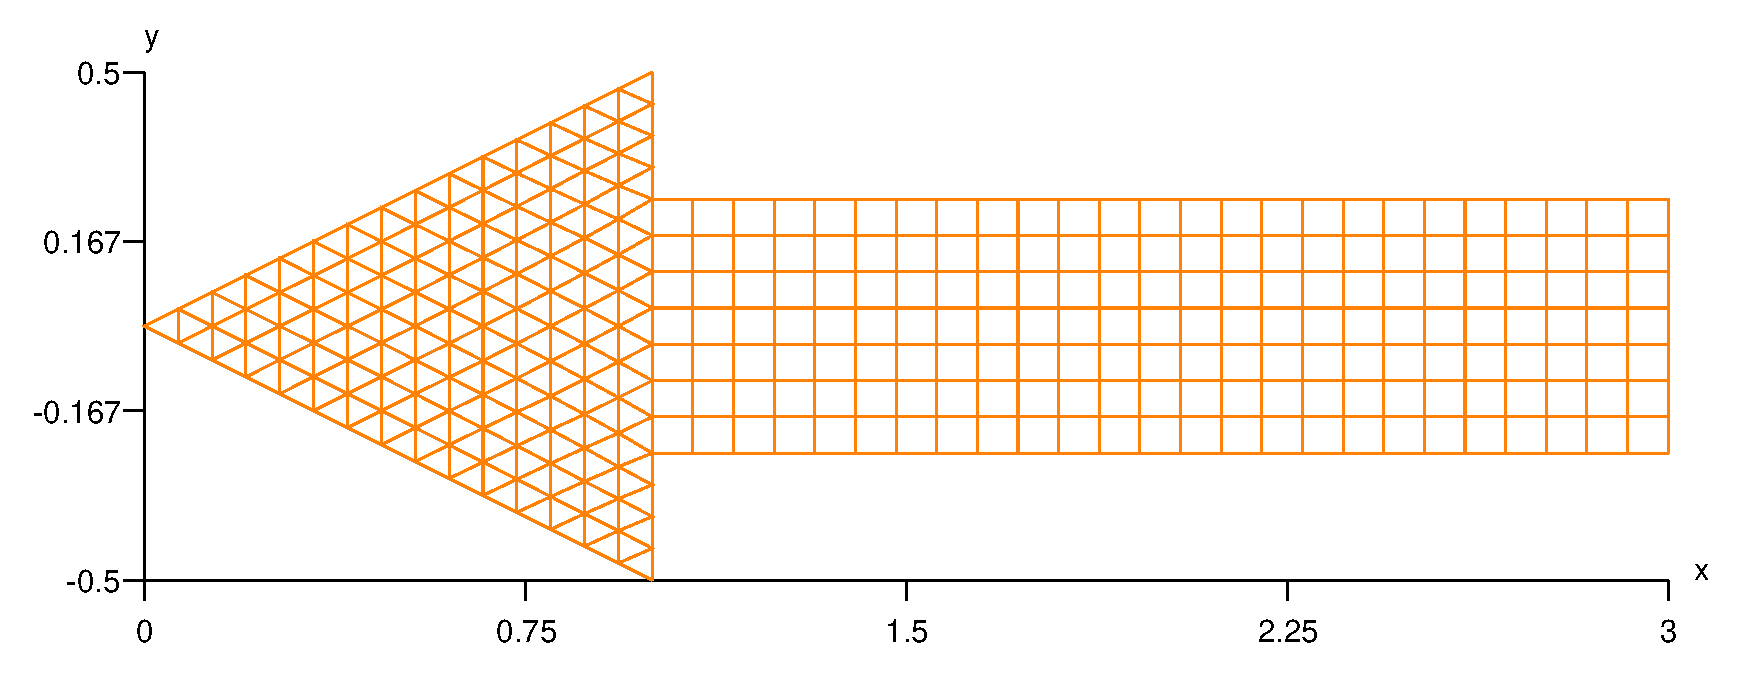
\includegraphics[width=135mm]{arrow}
  \caption{An arrow}
  \label{\numb section 2.\numb fig 2}
\end{figure}


          %-------------------------------%
\section{~~Triangular meshes on rectangles}\label{\numb section 2.\numb parag 3}
          %-------------------------------%

On a rectangular domain, we can build a mesh of triangles by using the {\small\tt \verm{Mesh}}
constructor with {\small\tt \verm{tag}::rectangle}, providing as last argument the
{\small\tt \verm{tag}::with\_\,triangles}.
For instance, in the example \ref{\numb section 1.\numb parag 3},
if we re-write the definition of {\small\tt BGHC} as

\begin{Verbatim}[commandchars=\\\{\},formatcom=\small\tt,baselinestretch=0.94]
   \verm{Mesh} \azul{BGHC} ( \verm{tag}::rectangle, BG, GH, HC, BC.reverse(), \verm{tag}::with_triangles );
\end{Verbatim}

\noindent we get the mesh shown in figure \ref{\numb section 2.\numb fig 3}.

\begin{figure}[ht] \centering
  \psfrag{A}{\tt\textcolor{textindraw}{A}}
  \psfrag{B}{\tt\textcolor{textindraw}{B}}
  \psfrag{C}{\tt\textcolor{textindraw}{C}}
  \psfrag{D}{\tt\textcolor{textindraw}{D}}
  \psfrag{E}{\tt\textcolor{textindraw}{E}}
  \psfrag{F}{\tt\textcolor{textindraw}{F}}
  \psfrag{G}{\tt\textcolor{textindraw}{G}}
  \psfrag{H}{\tt\textcolor{textindraw}{H}}
  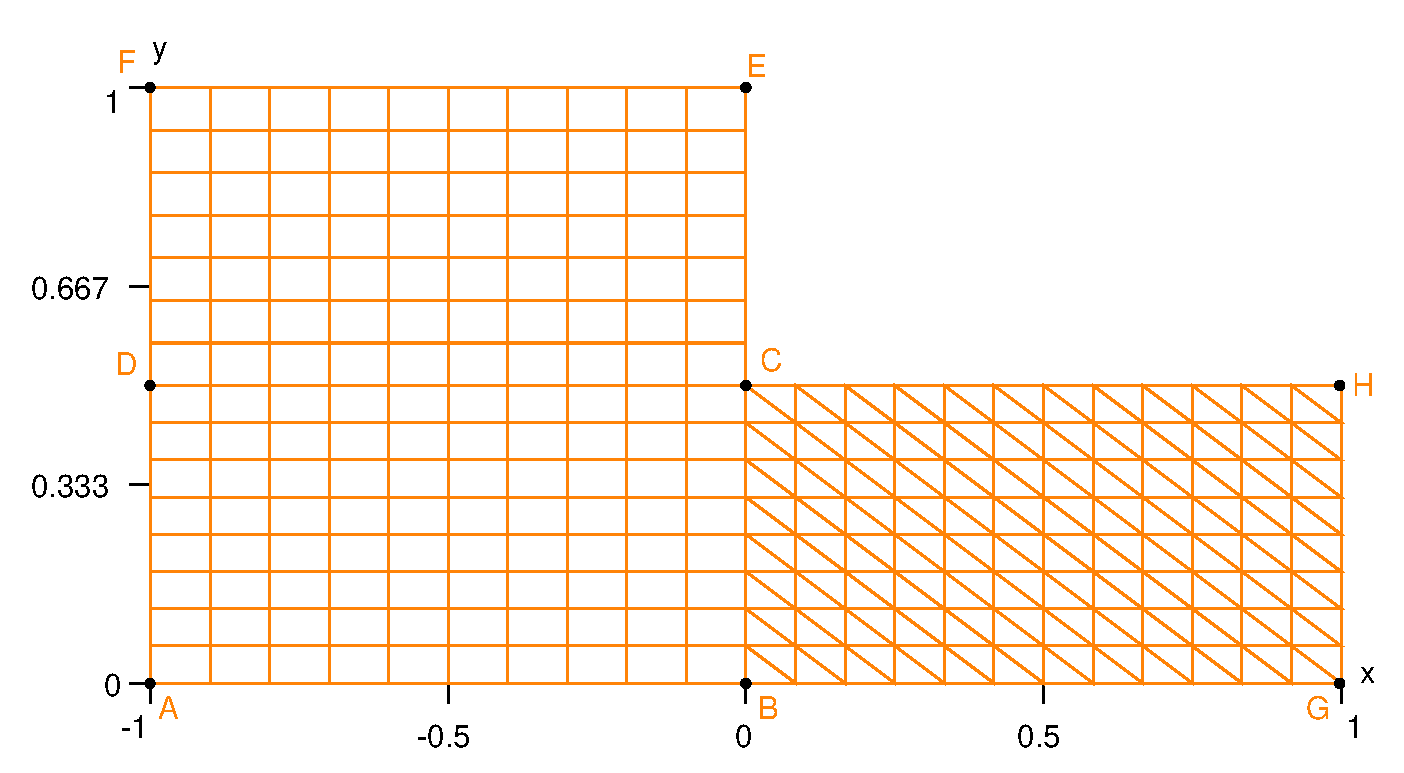
\includegraphics[width=115mm]{L-shaped-tri}
  \caption{An L-shaped mesh with triangular cells}
  \label{\numb section 2.\numb fig 3}
\end{figure}

If we give the sides of the rectangle in a different order, like in

\begin{Verbatim}[commandchars=\\\{\},formatcom=\small\tt,baselinestretch=0.94]
   \verm{Mesh} \azul{BGHC} ( \verm{tag}::rectangle, GH, HC, BC.reverse(), BG, \verm{tag}::with_triangles );
\end{Verbatim}

\noindent the rectangles will be cut along the other diagonal (check it yourself).

The mesh in paragraph \ref{\numb section 1.\numb parag 4} could have been built like this :

\begin{Verbatim}[commandchars=\\\{\},formatcom=\small\tt,baselinestretch=0.94]
   \verm{Mesh} \azul{ABD} ( \verm{tag}::triangle, AB, BD, AD.reverse() );
   \verm{Mesh} \azul{BCED} ( \verm{tag}::quadrangle, CE, ED, BD.reverse(), BC, \verm{tag}::with_triangles );
   \verm{Mesh} \azul{one_tri_one_rect} ( \verm{tag}::join, ABD, BCED );
\end{Verbatim}


          %-----------------------------------------------------%
\section{~~A manifold defined as a level set in $ \mathbb{R}^2 $}
          %-----------------------------------------------------%
\label{\numb section 2.\numb parag 4}

{\ManiFEM} allows one to define manifolds and submanifolds, and this feature may be
used to build domains of the desired shape.

Until now, we have only met the trivial Euclidian manifold, defined as {\small\tt
\verm{Manifold}\break ( \verm{tag}::Euclid,} {\small\tt \verm{tag}::of\_\,dim,} {\small\tt n}
{\small\tt )}.
One can define a submanifold in terms of an implicit equation, that is, as a level set,
using the method {\small\tt implicit} of the Euclidian manifold.
The code below introduces a one-dimensional submanifold of $ \mathbb{R}^2 $ (a hiperbola).

\begin{Verbatim}[commandchars=\\\{\},formatcom=\small\tt,frame=single,
   label=parag-\ref{\numb section 2.\numb parag 4}.cpp,rulecolor=\color{coment},
   baselinestretch=0.94,framesep=2mm]
   \verm{Manifold} \azul{RR2} ( \verm{tag}::Euclid, \verm{tag}::of_dim, 2 );
   \verm{Function} \azul{xy} = RR2.build_coordinate_system ( \verm{tag}::Lagrange, \verm{tag}::of_degree, 1 );
   \verm{Function} \azul{x} = xy[0],  \azul{y} = xy[1];
   
   \verm{Manifold} \azul{hiperbola} = RR2.implicit ( x*y == 1. );
   
   \verm{Cell} \azul{A} ( \verm{tag}::vertex );  x(A) =  0.5;   y(A) =  2.;
   \verm{Cell} \azul{B} ( \verm{tag}::vertex );  x(B) =  3;     y(B) =  0.333333333333;
   \verm{Mesh} \azul{arc_of_hiperbola} ( \verm{tag}::segment, A.reverse(), B, \verm{tag}::divided_in, 7 );
   arc_of_hiperbola.draw_ps (\verde{"hiperbola.eps"});
   arc_of_hiperbola.export_msh (\verde{"hiperbola.msh"});
\end{Verbatim}

\begin{figure}[ht] \centering
  \psfrag{A}{\tt\textcolor{textindraw}{A}}
  \psfrag{B}{\tt\textcolor{textindraw}{B}}
  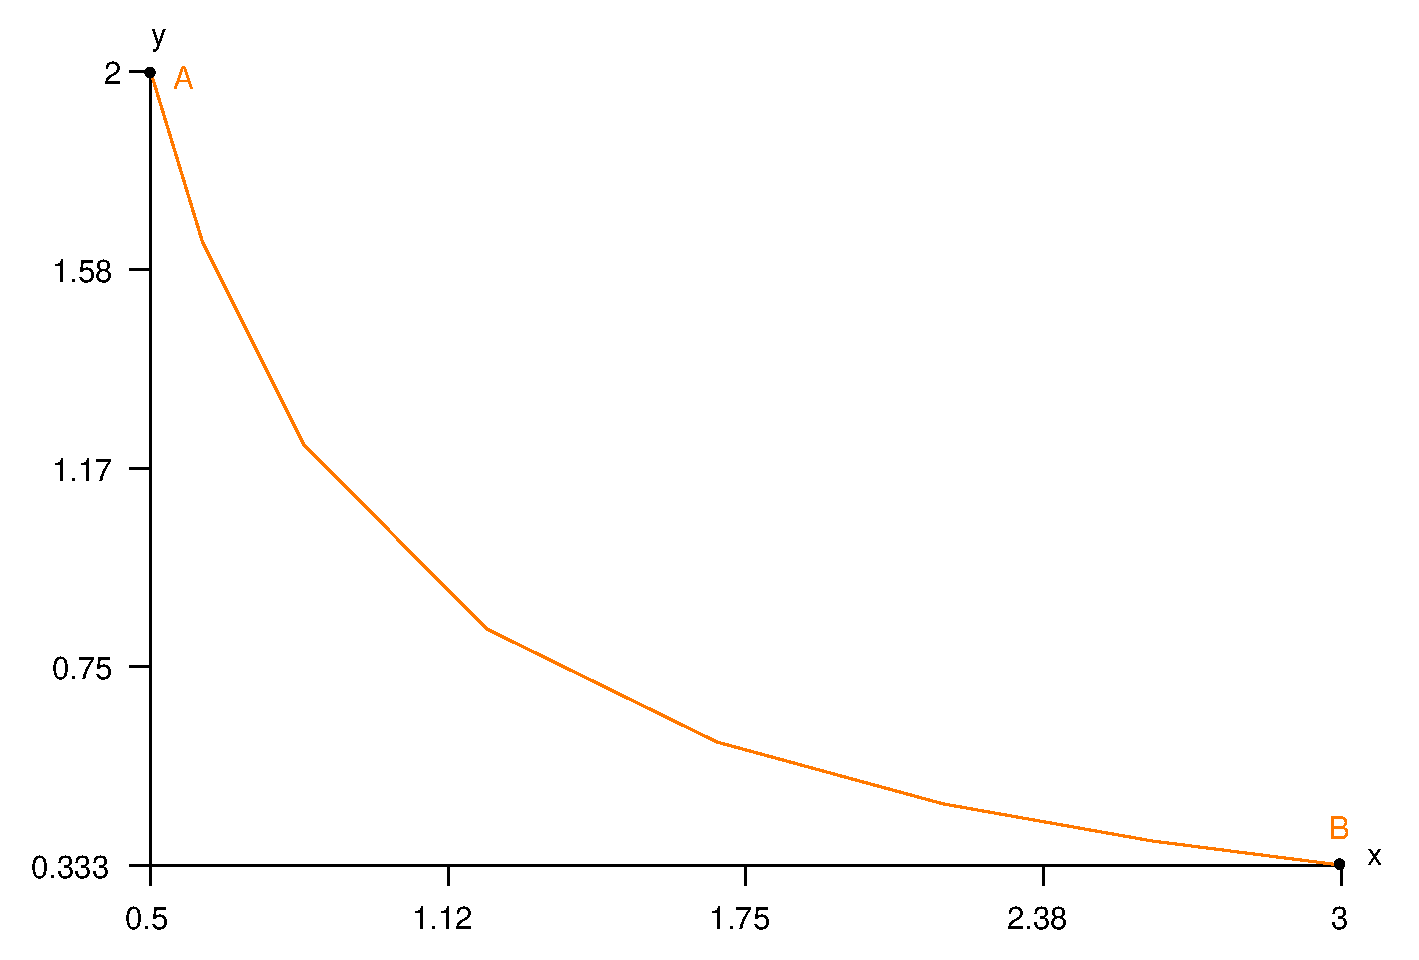
\includegraphics[width=105mm]{hiperbola}
  \caption{An arc of hiperbola}
  \label{\numb section 2.\numb fig 4}
\end{figure}

In {\tt gmsh}, you must select {\small\tt Tools} $\to$ {\small\tt Options} $\to$
{\small\tt Mesh} $\to$ {\small\tt 1D Elements} in order to see this mesh.

Note that the vertices are not perfectly uniformly distributed along the curve
because they are obtained as projections of points uniformly distributed along
the straight segment {\small\tt AB} onto the {\small\tt hiperbola} manifold.

Note also that when defining individual points {\small\tt A} and {\small\tt B} we must
be careful to set coordinates {\small\tt x} and {\small\tt y} within
the {\small\tt hiperbola} manifold.
As an alternative, we might explicitly project them onto the {\small\tt hiperbola} like this :

\begin{Verbatim}[commandchars=\\\{\},formatcom=\small\tt,baselinestretch=0.94]
   \verm{Cell} \azul{P} ( \verm{tag}::vertex );  x(P) = 0.6;   y(P) = 2.1;
   hiperbola.project(P);
\end{Verbatim}

\noindent In contrast, the {\small\tt \verm{Mesh}} constructor with {\small\tt \verm{tag}::segment}
builds points in the surrounding space {\small\tt RR2} and then projects them onto the
{\small\tt hiperbola} without the user's assistance.

The projection is done by applying a few steps of Newton's method for under-determined
(systems of) equations, as explained in paragraph \ref{\numb section 8.\numb parag 1}.

Paragraph \ref{\numb section 3.\numb parag 5} shows another way of meshing a curve,
producing equidistant vertices.


          %----------------------------------------%
\section{~~A circle defined by four curved segments}\label{\numb section 2.\numb parag 5}
          %----------------------------------------%

We can define several arcs of curve and {\small\tt join} them, thus obtaining a closed curve :
\medskip

\begin{Verbatim}[commandchars=\\\{\},formatcom=\small\tt,frame=single,
   label=parag-\ref{\numb section 2.\numb parag 5}.cpp,rulecolor=\color{coment},
   baselinestretch=0.94,framesep=2mm]
   \verm{Manifold} \azul{circle_manifold} = RR2.implicit ( x*x + y*y == 1. );
   \verm{Cell} \azul{N} ( \verm{tag}::vertex );  x(N) =  0.;   y(N) =  1.;
   \verm{Cell} \azul{W} ( \verm{tag}::vertex );  x(W) = -1.;   y(W) =  0.;
   \verm{Cell} \azul{S} ( \verm{tag}::vertex );  x(S) =  0.;   y(S) = -1.;
   \verm{Cell} \azul{E} ( \verm{tag}::vertex );  x(E) =  1.;   y(E) =  0.;
   \verm{Mesh} \azul{NW} ( \verm{tag}::segment, N.reverse(), W, \verm{tag}::divided_in, 5 );
   \verm{Mesh} \azul{WS} ( \verm{tag}::segment, W.reverse(), S, \verm{tag}::divided_in, 5 );
   \verm{Mesh} \azul{SE} ( \verm{tag}::segment, S.reverse(), E, \verm{tag}::divided_in, 5 );
   \verm{Mesh} \azul{EN} ( \verm{tag}::segment, E.reverse(), N, \verm{tag}::divided_in, 5 );
   \verm{Mesh} \azul{circle} ( \verm{tag}::join, NW, WS, SE, EN );
\end{Verbatim}

\begin{figure}[ht] \centering
  \psfrag{N}{\tt\textcolor{textindraw}{N}}
  \psfrag{S}{\tt\textcolor{textindraw}{S}}
  \psfrag{E}{\tt\textcolor{textindraw}{E}}
  \psfrag{W}{\tt\textcolor{textindraw}{W}}
  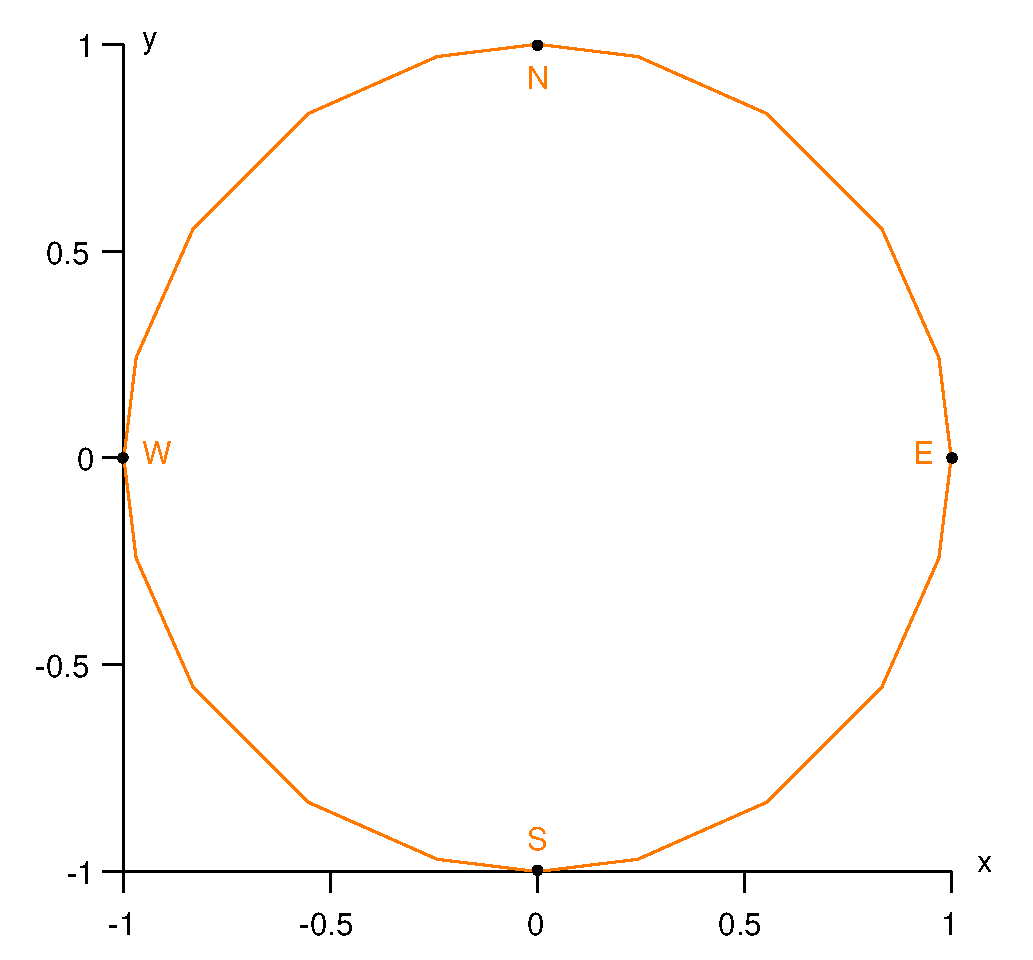
\includegraphics[width=80mm]{circle}
  \caption{A circle obtained by {\small\tt join}ing four segments}
  \label{\numb section 2.\numb fig 5}
\end{figure}

Again, the distribution of vertices along the circle is not perfect
because vertices are obtained as projections (on the circle) of points
along straight segments {\small\tt NW}, {\small\tt WS} and so forth.
Paragraph \ref{\numb section 3.\numb parag 2} shows another way of meshing a closed curve,
producing equidistant vertices.

Note that applying the {\small\tt \verm{Mesh}} constructor with {\small\tt \verm{tag}::join}
to four segments is very different from applying the {\small\tt \verm{Mesh}} constructor with
{\small\tt \verm{tag}::quadrangle} to the same four segments;
see paragraphs \ref{\numb section 2.\numb parag 9} and \ref{\numb section 2.\numb parag 10}.


          %---------------------------------------------%
\section{~~A hemisphere defined by four curved triangles}\label{\numb section 2.\numb parag 6}
          %---------------------------------------------%

Let's look at a surface in $ \mathbb{R}^3 $ :

\begin{Verbatim}[commandchars=\\\{\},formatcom=\small\tt,frame=single,
   label=parag-\ref{\numb section 2.\numb parag 6}.cpp,rulecolor=\color{coment},
   baselinestretch=0.94,framesep=2mm                                            ]
   \verm{Manifold} \azul{RR3} ( \verm{tag}::Euclid, \verm{tag}::of_dim, 3 );
   \verm{Function} \azul{xyz} = RR3.build_coordinate_system ( \verm{tag}::Lagrange, \verm{tag}::of_degree, 1 );
   \verm{Function} \azul{x} = xyz[0],  \azul{y} = xyz[1],  \azul{z} = xyz[2];

   \verm{Manifold} \azul{sphere} = RR3.implicit ( x*x + y*y + z*z == 1. );
   \cinza{// let's mesh half of a sphere}
   \verm{Cell} \azul{E}  ( \verm{tag}::vertex );   x(E) =  1.;   y(E) =  0.;   z(E) = 0.;
   \verm{Cell} \azul{N}  ( \verm{tag}::vertex );   x(N) =  0.;   y(N) =  1.;   z(N) = 0.;
   \verm{Cell} \azul{W}  ( \verm{tag}::vertex );   x(W) = -1.;   y(W) =  0.;   z(W) = 0.;
   \verm{Cell} \azul{S}  ( \verm{tag}::vertex );   x(W) =  0.;   y(W) = -1.;   z(W) = 0.;
   \verm{Cell} \azul{up} ( \verm{tag}::vertex );   x(up)=  0.;   y(up)=  0.;   z(up)= 1.;
   int \azul{n} = 15;
   \verm{Mesh} \azul{EN} ( \verm{tag}::segment, E.reverse(), N, \verm{tag}::divided_in, n );
   \verm{Mesh} \azul{NW} ( \verm{tag}::segment, N.reverse(), W, \verm{tag}::divided_in, n );
   \verm{Mesh} \azul{WS} ( \verm{tag}::segment, W.reverse(), S, \verm{tag}::divided_in, n );
   \verm{Mesh} \azul{SE} ( \verm{tag}::segment, S.reverse(), E, \verm{tag}::divided_in, n );
   \verm{Mesh} \azul{upE} ( \verm{tag}::segment, up.reverse(), E, \verm{tag}::divided_in, n );
   \verm{Mesh} \azul{upN} ( \verm{tag}::segment, up.reverse(), N, \verm{tag}::divided_in, n );
   \verm{Mesh} \azul{upW} ( \verm{tag}::segment, up.reverse(), W, \verm{tag}::divided_in, n );
   \verm{Mesh} \azul{upS} ( \verm{tag}::segment, up.reverse(), S, \verm{tag}::divided_in, n );
\end{Verbatim}

\begin{figure}[ht] \centering
  \psfrag{S}{\tt\textcolor{textindraw}{S}}
  \psfrag{W}{\tt\textcolor{textindraw}{W}}
  \psfrag{up}{\tt\textcolor{textindraw}{up}}
  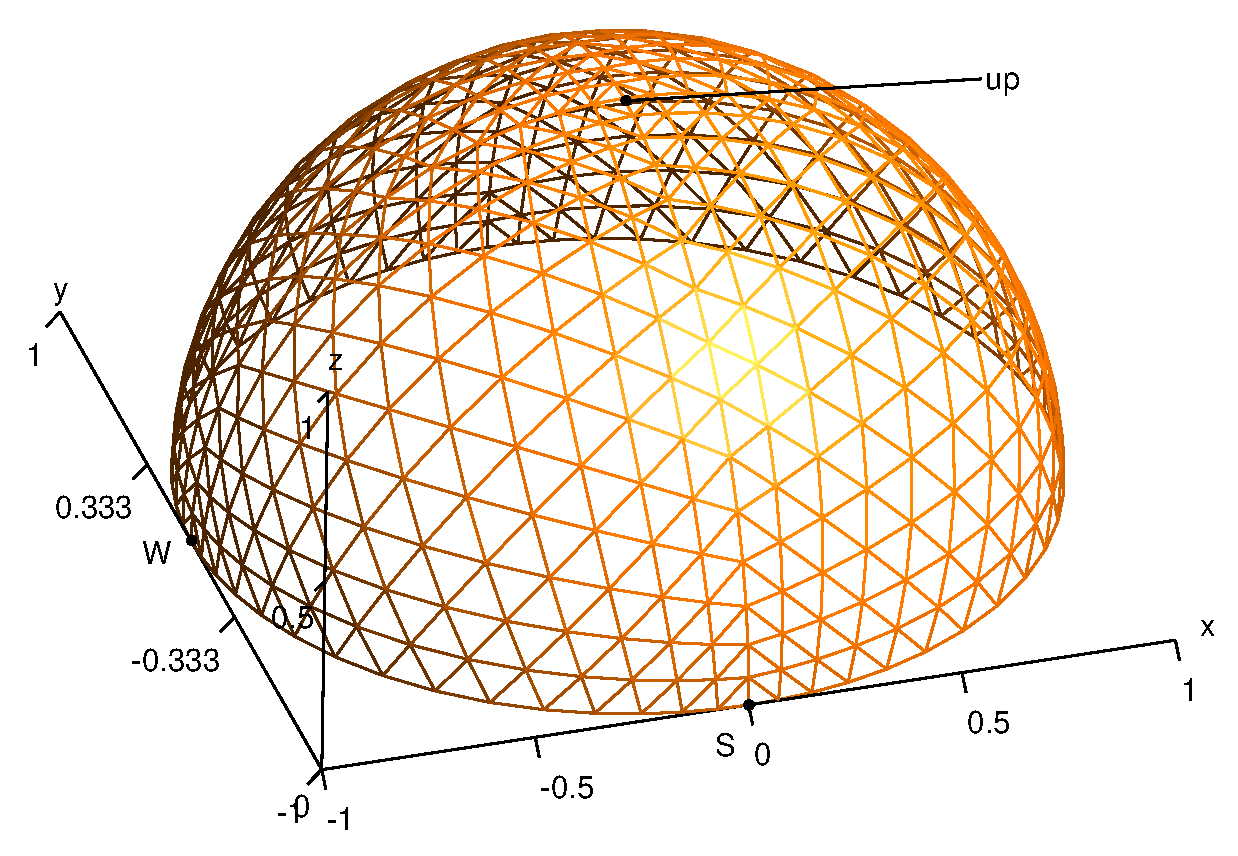
\includegraphics[width=105mm]{hemisphere}
  \caption{A hemisphere obtained by {\small\tt join}ing four triangles}
\end{figure}

\begin{Verbatim}[commandchars=\\\{\},formatcom=\small\tt,frame=single,
   label=parag-\ref{\numb section 2.\numb parag 6}.cpp,rulecolor=\color{coment},
   baselinestretch=0.94,framesep=2mm                                            ]
   \cinza{// build four triangles}
   \verm{Mesh} \azul{ENup} ( \verm{tag}::triangle, EN, upN.reverse(), upE );
   \verm{Mesh} \azul{NWup} ( \verm{tag}::triangle, NW, upW.reverse(), upN );
   \verm{Mesh} \azul{WSup} ( \verm{tag}::triangle, WS, upS.reverse(), upW );
   \verm{Mesh} \azul{SEup} ( \verm{tag}::triangle, SE, upE.reverse(), upS );

   \cinza{// and finally join the triangles :}
   \verm{Mesh} \azul{hemisphere} ( \verm{tag}::join, ENup, NWup, WSup, SEup );
\end{Verbatim}

Again, when we define individual points {\small\tt E}, {\small\tt N}, {\small\tt W},
{\small\tt S} and {\small\tt up} we must be careful to provide coordinates on the
{\small\tt sphere} (or {\small\tt project} them explicitly as shown in paragraph
\ref{\numb section 2.\numb parag 7}).
In contrast, the {\small\tt \verm{Mesh}} constructors with {\small\tt \verm{tag}::segment},
{\small\tt \verm{tag}::quadrangle} and {\small\tt \verm{tag}::triangle} build points in the
surrounding space ($ \mathbb{R}^2 $ or $ \mathbb{R}^3 $) and
then project them onto the current manifold without the user's assistance (paragraph
\ref{\numb section 8.\numb parag 1} describes this projection operation).
As a side effect, within each triangle ({\small\tt ENup}, {\small\tt NWup} and so forth),
the distribution of the vertices is not perfectly uniform.

Note that, when we build the segments {\small\tt WS}, {\small\tt upS} and so on,
we know that those segments will be (polygonal approximations of) arcs of circle on the sphere.
This is so due to the particular geometry of our manifold (we know that the projection of
a straight line segment on the sphere is an arc of circle of radius equal to the radius of
the sphere); the shape of such segments is less clear in other examples
(like the one in paragraph \ref{\numb section 2.\numb parag 7}).

Section \ref{\numb section 3} shows other ways of meshing a surface.


          %----------------------%
\section{~~A more complex surface}\label{\numb section 2.\numb parag 7}
          %----------------------%

If the surface is more ``bumpy'',
% since the projection operation doesn't work well for points far from the manifold,
we must use smaller patches in order to get a mesh of good quality.

Below we use twelve rectangles to get a bumpy hemisphere.

\begin{Verbatim}[commandchars=\\\{\},formatcom=\small\tt,frame=single,
   label=parag-\ref{\numb section 2.\numb parag 7}.cpp,rulecolor=\color{coment},
   baselinestretch=0.94,framesep=2mm]
   \verm{Manifold} nut = RR3.implicit ( x*x + y*y + z*z + 1.5*x*y*z == 1. );

   \cinza{// let's mesh a hemisphere (much deformed)}
   \verm{Cell} \azul{S} ( \verm{tag}::vertex );    x(S)  =   0.;   y(S)  =  -1.;   z(S)  =  0.;
   \verm{Cell} \azul{E} ( \verm{tag}::vertex );    x(E)  =   1.;   y(E)  =   0.;   z(E)  =  0.;
   \verm{Cell} \azul{N} ( \verm{tag}::vertex );    x(N)  =   0.;   y(N)  =   1.;   z(N)  =  0.;
   \verm{Cell} \azul{W} ( \verm{tag}::vertex );    x(W)  =  -1.;   y(W)  =   0.;   z(W)  =  0.;
   \verm{Cell} \azul{up} ( \verm{tag}::vertex );   x(up) =   0.;   y(up) =   0.;   z(up) =  1.;
   \cinza{// no need to project these}
   \verm{Cell} \azul{mSW} ( \verm{tag}::vertex );  x(mSW) = -1.;   y(mSW) = -1.;   z(mSW) = 0.;
   nut.project ( mSW );  \cinza{// midway between S and W}
   \verm{Cell} \azul{mSup}  ( \verm{tag}::vertex );  x(mSup) =  0.;   y(mSup) = -1.;   z(mSup) = 1.;
   nut.project ( mSup );  \cinza{// midway between S and up}
   \verm{Cell} \azul{mSWup} ( \verm{tag}::vertex );  x(mSWup) = -1.;  y(mSWup) = -1.;  z(mSWup) = 1.;
   nut.project ( mSWup );  \cinza{// somewhere between S, W and up}
   \cinza{// ... and so forth ...}

   \cinza{// now build segments :}
   int \azul{n} = 10;
   \verm{Mesh} \azul{W_mSW}  ( \verm{tag}::segment, W.reverse(), mSW,  \verm{tag}::divided_in, n );
   \verm{Mesh} \azul{W_mWup} ( \verm{tag}::segment, W.reverse(), mWup, \verm{tag}::divided_in, n );
   \cinza{// ... and so forth ...}
\end{Verbatim}

\begin{figure}[ht] \centering
  \psfrag{S}{\tt\textcolor{textindraw}{S}}
  \psfrag{W}{\tt\textcolor{textindraw}{W}}
  \psfrag{mWS}{\tt\textcolor{textindraw}{mWS}}
  \psfrag{mSE}{\tt\textcolor{textindraw}{mSE}}
  \psfrag{mWup}{\tt\textcolor{textindraw}{mWup}}
  \psfrag{mSup}{\tt\textcolor{textindraw}{mSup}}
  \psfrag{mSEup}{\tt\textcolor{textindraw}{mSEup}}
  \psfrag{up}{\tt\textcolor{textindraw}{up}}
  \psfrag{mWSup}{\tt\textcolor{textindraw}{mWSup}}
  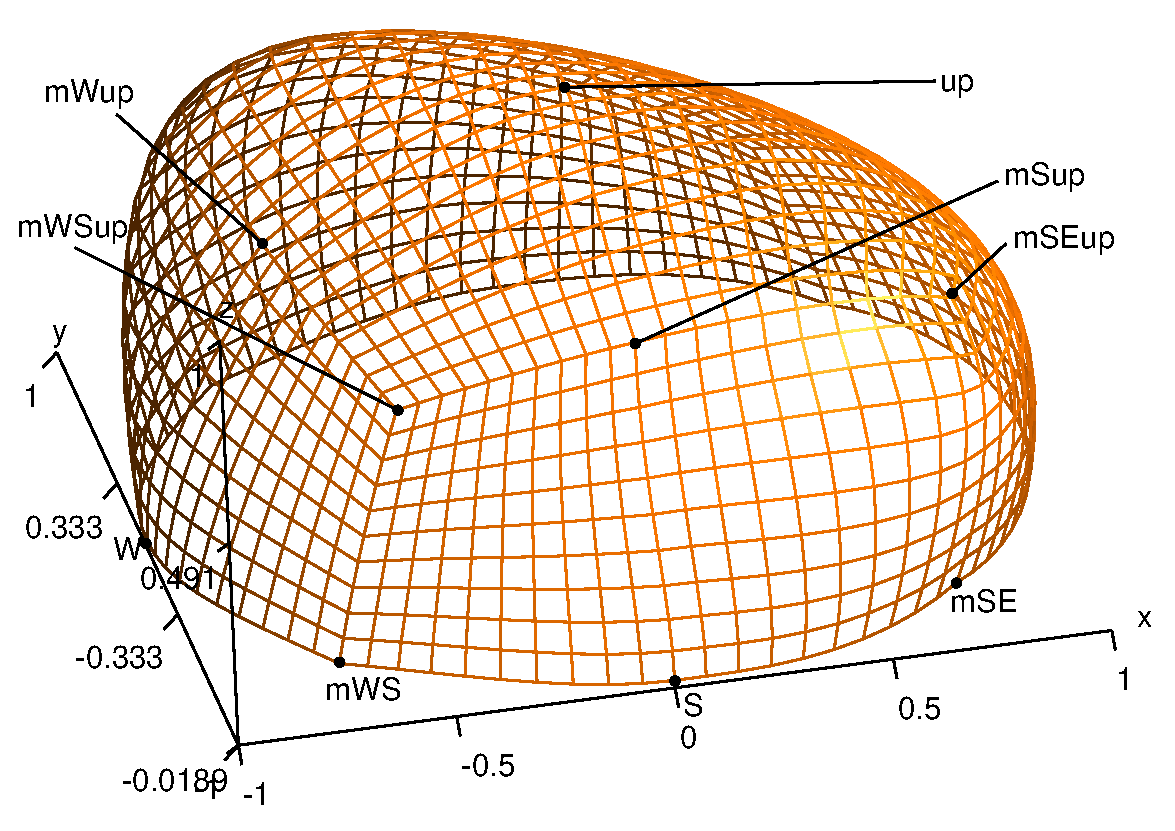
\includegraphics[width=110mm]{hemisphere-2}
  \caption{Here we have {\small\tt join}ed twelve rectangles}
  \label{\numb section 2.\numb fig 7}
\end{figure}
	
\begin{Verbatim}[commandchars=\\\{\},formatcom=\small\tt,frame=single,
   label=parag-\ref{\numb section 2.\numb parag 7}.cpp,rulecolor=\color{coment},
   baselinestretch=0.94,framesep=2mm]
   \cinza{// now the twelve rectangles :}
   \verm{Mesh} \azul{rect_W_SW}  ( \verm{tag}::quadrangle,
      mSW_mSWup, mWup_mSWup.reverse(), W_mWup.reverse(), W_mSW );
   \verm{Mesh} \azul{rect_S_SW}  ( \verm{tag}::quadrangle,
      mSup_mSWup, mSW_mSWup.reverse(), S_mSW.reverse(), S_mSup );
   \verm{Mesh} \azul{rect_up_SW} ( \verm{tag}::quadrangle,
      mWup_mSWup, mSup_mSWup.reverse(), up_mSup.reverse(), up_mWup );
   \cinza{// ... and so forth ...}

   \cinza{// and finally join the rectangles :}
   \verm{Mesh} \azul{hemisphere} ( \verm{tag}::join,
      \{ rect_E_NE, rect_E_SE, rect_S_SE, rect_S_SW, rect_W_SW, rect_W_NW,
        rect_N_NE, rect_N_NW, rect_up_SE, rect_up_SW, rect_up_NE, rect_up_NW \} );
\end{Verbatim}

Note how we use a version of the {\small\tt \verm{Mesh}} constructor with {\small\tt \verm{tag}::join}
taking as argument a list of {\small\tt \verm{Mesh}}es; the same constructor is used in
paragraph \ref{\numb section 9.\numb parag 2}.

Unlike in paragraph \ref{\numb section 2.\numb parag 6}, here we do not control the
exact shape of the segments {\small\tt S\_\,mSW}, {\small\tt S\_\,mSup} and so on.
They are projections of straight line segments onto our surface but since the equation
of the surface is rather complicated we do not know the exact shape of these projections.
Since points like {\small\tt mSW} and {\small\tt mSE} have been placed initially in
{\small\tt RR3} not belonging to the {\small\tt bupmy} manifold and then explicitly
{\small\tt project}ed,
there is no guarantee that they lie in the plane $ z = 0 $ (they probably don't).
We notice an angle between {\small\tt W\_\,mSW} and {\small\tt S\_\,mSW} at {\small\tt mSW}.

Paragraph \ref{\numb section 2.\numb parag 13} shows a way to control the shape of the segments
{\small\tt S\_\,mSW}, {\small\tt S\_\,mSE} and so on.

Section \ref{\numb section 3} shows other ways of meshing a surface.


          %--------%
\section{~~Exercise}\label{\numb section 2.\numb parag 8}
          %--------%

Slightly change the code in paragraph \ref{\numb section 2.\numb parag 7}
in order to obtain the mesh shown in figure \ref{\numb section 2.\numb fig 8}.
(Hint: have a look at paragraph \ref{\numb section 2.\numb parag 3}.)

\begin{figure}[ht] \centering
  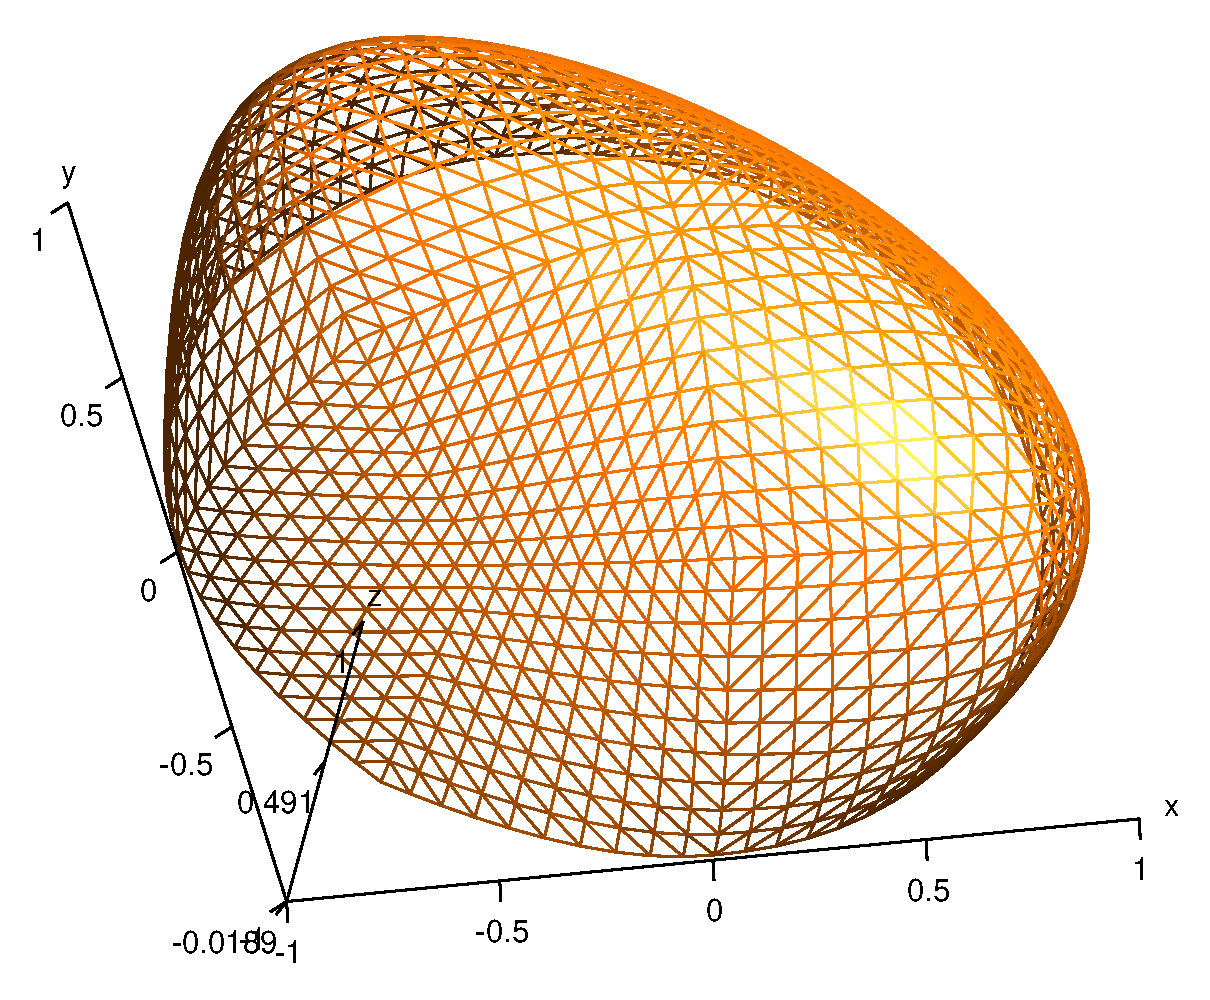
\includegraphics[width=110mm]{hemisphere-1}
  \caption{Using triangular cells}
  \label{\numb section 2.\numb fig 8}
\end{figure}


          %-----------------------------%
\section{~~Alternating between manifolds}\label{\numb section 2.\numb parag 9}
          %-----------------------------%

Let's go back to the example in paragraph \ref{\numb section 2.\numb parag 5}.
Suppose we want to mesh the whole disk, not just its boundary.
We can build the boundary of the disk just like in paragraph
\ref{\numb section 2.\numb parag 5}, by placing ourselves in the manifold {\small\tt circle}.
But if we want to subsequently mesh the interior of the disk, we must leave {\small\tt circle}
and switch back to the original {\small\tt RR2} manifold.
Method {\small\tt set\_\,as\_\,working\_\,manifold} allows us to do that.

\begin{Verbatim}[commandchars=\\\{\},formatcom=\small\tt,frame=single,
   label=parag-\ref{\numb section 2.\numb parag 9}.cpp,rulecolor=\color{coment},
   baselinestretch=0.94,framesep=2mm]
   \verm{Manifold} \azul{RR2} ( \verm{tag}::Euclid, \verm{tag}::of_dim, 2 );
   \verm{Function} \azul{xy} = RR2.build_coordinate_system ( \verm{tag}::Lagrange, \verm{tag}::of_degree, 1 );
   \verm{Function} \azul{x} = xy[0],  \azul{y} = xy[1];
   
   \verm{Manifold} \azul{circle} = RR2.implicit ( x*x + y*y == 1. );
   
   \verm{Cell} \azul{N} ( \verm{tag}::vertex );  x(N) =  0.;   y(N) =  1.;
   \verm{Cell} \azul{W} ( \verm{tag}::vertex );  x(W) = -1.;   y(W) =  0.;
   \verm{Cell} \azul{S} ( \verm{tag}::vertex );  x(S) =  0.;   y(S) = -1.;
   \verm{Cell} \azul{E} ( \verm{tag}::vertex );  x(E) =  1.;   y(E) =  0.;
   \verm{Mesh} \azul{NW} ( \verm{tag}::segment, N.reverse(), W, \verm{tag}::divided_in, 10 );
   \verm{Mesh} \azul{WS} ( \verm{tag}::segment, W.reverse(), S, \verm{tag}::divided_in, 10 );
   \verm{Mesh} \azul{SE} ( \verm{tag}::segment, S.reverse(), E, \verm{tag}::divided_in, 10 );
   \verm{Mesh} \azul{EN} ( \verm{tag}::segment, E.reverse(), N, \verm{tag}::divided_in, 10 );
   
   RR2.set_as_working_manifold();
   \verm{Mesh} \azul{disk} ( \verm{tag}::quadrangle, NW, WS, SE, EN );
\end{Verbatim}

\begin{figure}[ht] \centering
  \psfrag{S}{\tt\textcolor{textindraw}{S}}
  \psfrag{N}{\tt\textcolor{textindraw}{N}}
  \psfrag{E}{\tt\textcolor{textindraw}{E}}
  \psfrag{W}{\tt\textcolor{textindraw}{W}}
  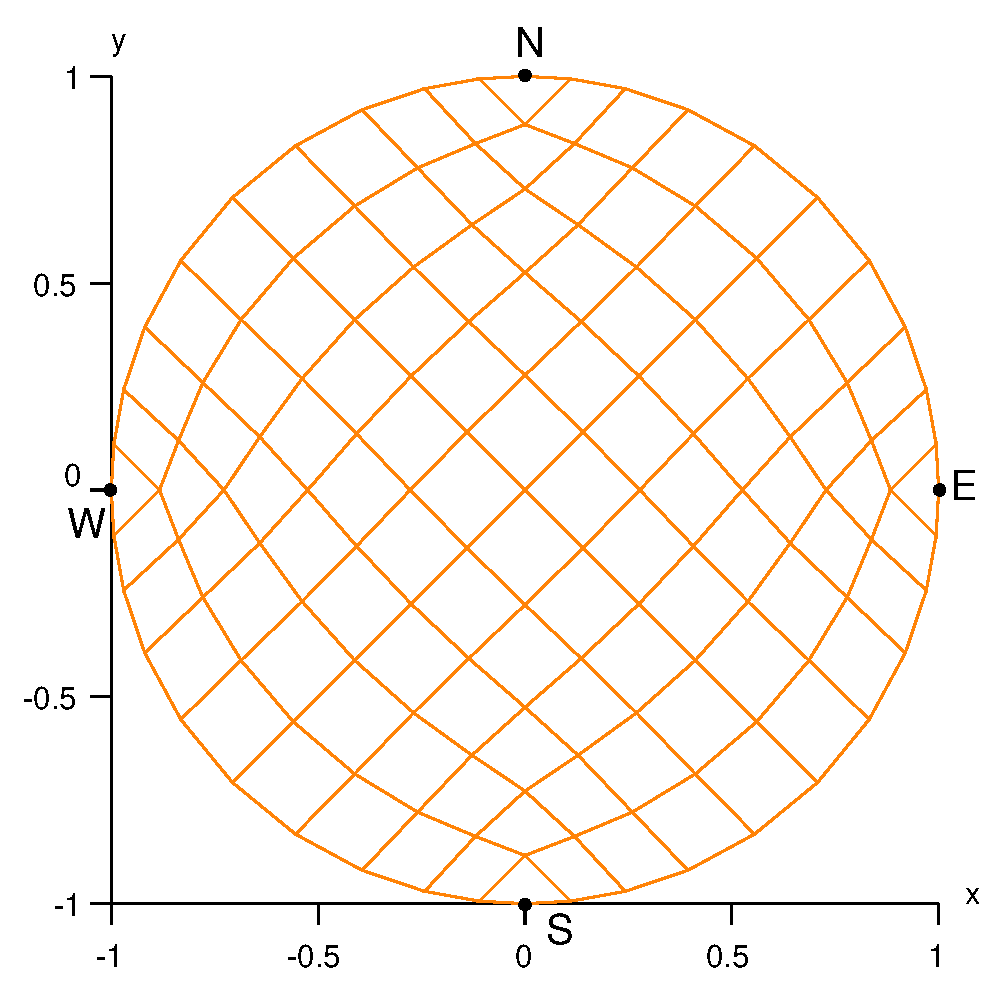
\includegraphics[width=70mm]{disk}
  \caption{A disk treated as a rectangle}
  \label{\numb section 2.\numb fig 9}
\end{figure}

The mesh (shown in figure \ref{\numb section 2.\numb fig 9}) is of poor quality;
we obtain quadrilaterals having a wide angle near {\small\tt S}, {\small\tt N}, {\small\tt E}
and {\small\tt W}.
Paragraphs \ref{\numb section 3.\numb parag 1} and \ref{\numb section 3.\numb parag 2} show
another way of meshing a disk, having its boundary as starting point.

Each time a {\small\tt \verm{Manifold}} object is created, its constructor sets it as working manifold;
this is why in many cases we don't need to know about method
{\small\tt set\_\,as\_\,working\_\,manifold}.
We need it, however, in cases like the one presented here.


          %------------------------------------%
\section{~~Alternating between manifolds, again}\label{\numb section 2.\numb parag 10}
          %------------------------------------%

Here is an example similar to the one in paragraph \ref{\numb section 2.\numb parag 9},
this time with four arcs of hiperbola.

\begin{figure}[ht] \centering
  \psfrag{S}{\tt\textcolor{textindraw}{S}}
  \psfrag{N}{\tt\textcolor{textindraw}{N}}
  \psfrag{E}{\tt\textcolor{textindraw}{E}}
  \psfrag{W}{\tt\textcolor{textindraw}{W}}
  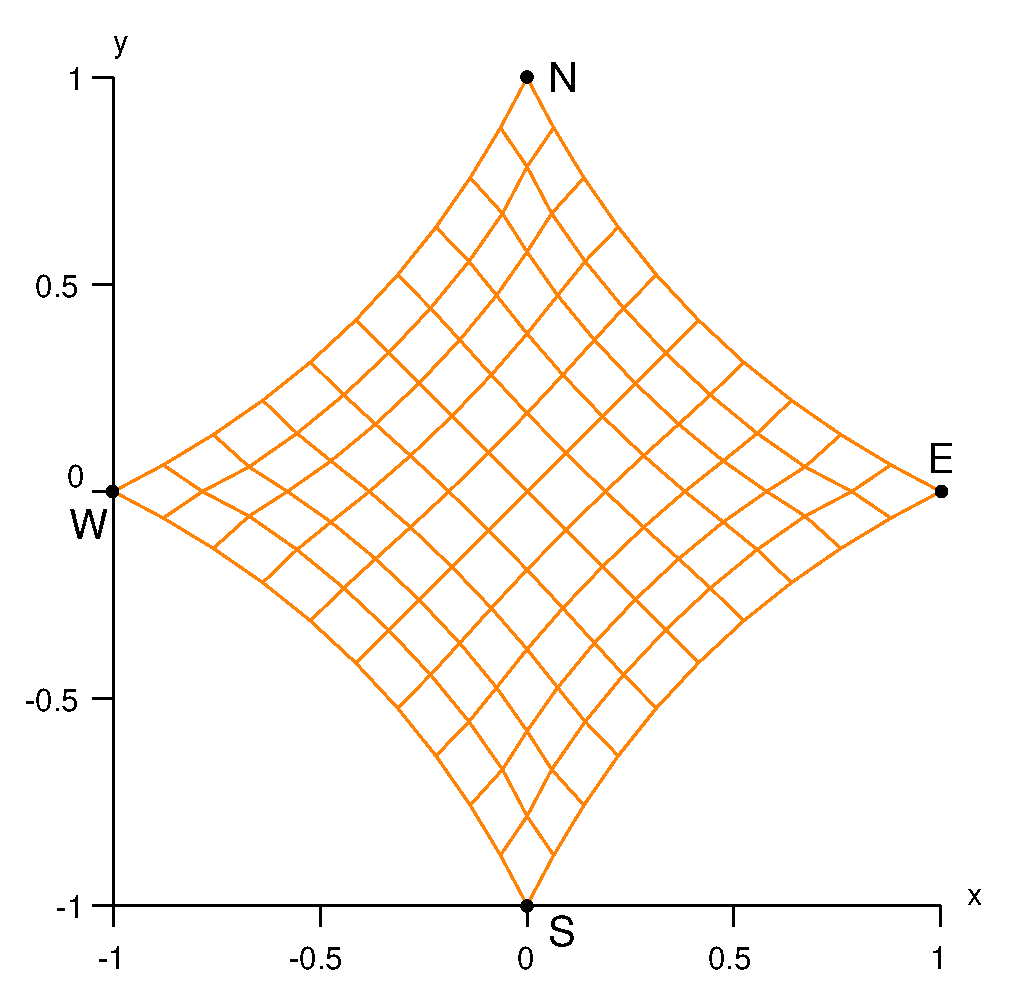
\includegraphics[width=80mm]{diamond}
  \caption{A diamond shape}
  \label{\numb section 2.\numb fig 10}
\end{figure}

\begin{Verbatim}[commandchars=\\\{\},formatcom=\small\tt,frame=single,
   label=parag-\ref{\numb section 2.\numb parag 10}.cpp,rulecolor=\color{coment},
   baselinestretch=0.94,framesep=2mm]
   \verm{Manifold} \azul{RR2} ( \verm{tag}::Euclid, \verm{tag}::of_dim, 2 );
   \verm{Function} \azul{xy} = RR2.build_coordinate_system ( \verm{tag}::Lagrange, \verm{tag}::of_degree, 1 );
   \verm{Function} \azul{x} = xy[0],  \azul{y} = xy[1];
   \verm{Cell} \azul{N} ( \verm{tag}::vertex );  x(N) =  0.;   y(N) =  1.;
   \verm{Cell} \azul{W} ( \verm{tag}::vertex );  x(W) = -1.;   y(W) =  0.;
   \verm{Cell} \azul{S} ( \verm{tag}::vertex );  x(S) =  0.;   y(S) = -1.;
   \verm{Cell} \azul{E} ( \verm{tag}::vertex );  x(E) =  1.;   y(E) =  0.;

   \verm{Manifold} \azul{first_arc}  = RR2.implicit ( x*y + x - y == -1. );
   \verm{Mesh} \azul{NW} ( \verm{tag}::segment, N.reverse(), W, \verm{tag}::divided_in, 10 );
   \verm{Manifold} \azul{second_arc} = RR2.implicit ( x*y - x - y ==  1. );
   \verm{Mesh} \azul{WS} ( \verm{tag}::segment, W.reverse(), S, \verm{tag}::divided_in, 10 );
   \verm{Manifold} \azul{third_arc}  = RR2.implicit ( x*y - x + y == -1. );
   \verm{Mesh} \azul{SE} ( \verm{tag}::segment, S.reverse(), E, \verm{tag}::divided_in, 10 );
   \verm{Manifold} \azul{fourth_arc} = RR2.implicit ( x*y + x + y ==  1. );
   \verm{Mesh} \azul{EN} ( \verm{tag}::segment, E.reverse(), N, \verm{tag}::divided_in, 10 );
   
   RR2.set_as_working_manifold();
   \verm{Mesh} \azul{diamond} ( \verm{tag}::quadrangle, NW, WS, SE, EN );
\end{Verbatim}

Paragraph \ref{\numb section 3.\numb parag 17} shows another way of meshing the same domain.


          %----------------%
\section{~~An organic shape}\label{\numb section 2.\numb parag 11}
          %----------------%

This paragraph describes a surface meant to mimic the shape of a physalis fruit.

%\begin{figure}[h!]\centering
%  
\includegraphics[width=85mm]{empty}
%  \caption{Dry physalis, with fruit inside}\label{\numb section 2.\numb fig 11}
%\end{figure}

\begin{figure}[ht]\centering
%\vskip -3mm
\if\production 1
\centerline{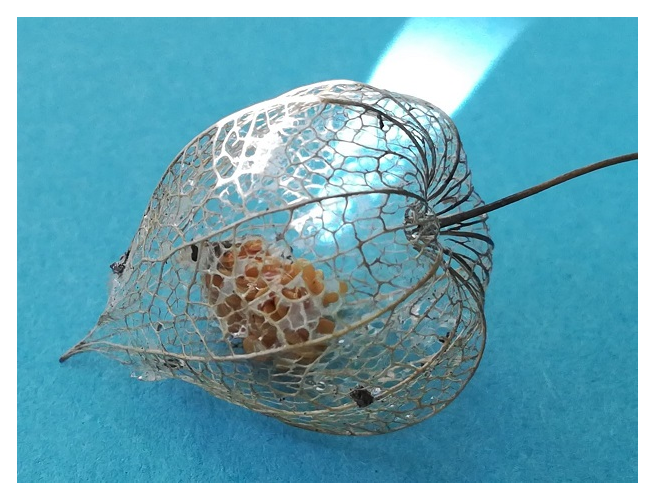
\includegraphics[width=85mm]{dry-physalis}}
\else
\psfrag{photo}{[photo of a physalis]}
\centerline{
\includegraphics[width=95mm]{fake-physalis}}
\fi
  \caption{Dry physalis, with fruit inside}\label{\numb section 2.\numb fig 11}
\end{figure}
%\vfil\eject

We begin by defining a revolution surface in $ \mathbb{R}^3 $ :

\begin{Verbatim}[commandchars=\\\{\},formatcom=\small\tt,frame=single,
   label=parag-\ref{\numb section 2.\numb parag 11}.cpp,rulecolor=\color{coment},
   baselinestretch=0.94,framesep=2mm]
   \verm{Function} \azul{r2} = x*x + y*y + z*z;
   const double \azul{pi} = 3.1415926536;
   \verm{Manifold} \azul{apple} = RR3.implicit ( \verm{power}(r2,0.5) * \verm{sin}(r2-pi/6.) == z );
\end{Verbatim}

This surface has the shape shown in figure \ref{\numb section 2.\numb fig 12},
which does not resemble a physalis fruit.

\begin{figure}[ht] \centering
  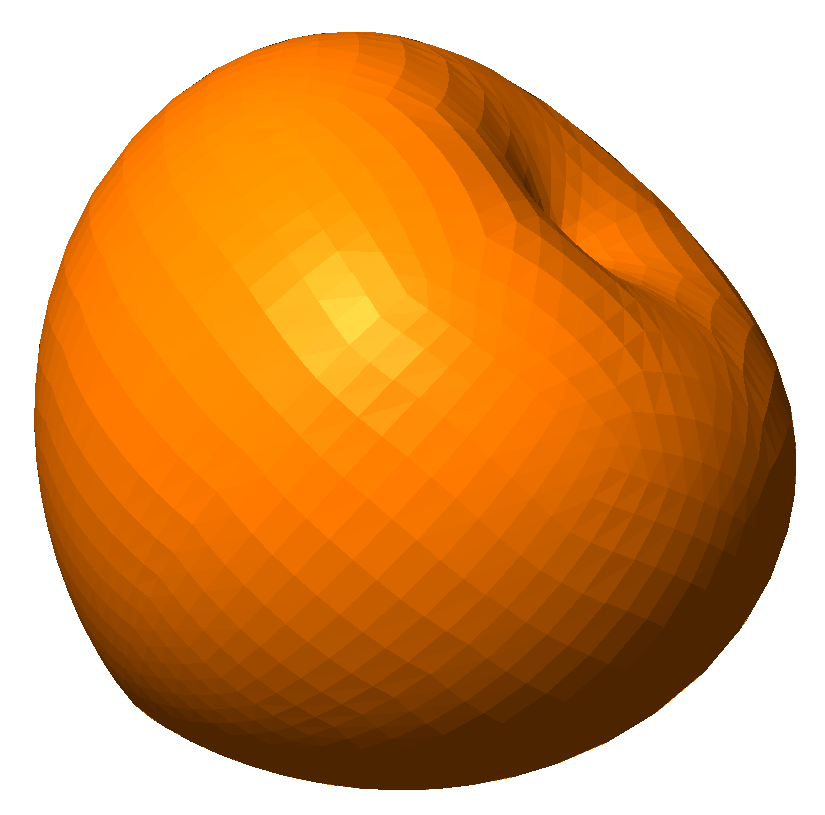
\includegraphics[width=80mm]{fisalis-manif}
  \caption{A compact manifold resembling an apple}
  \label{\numb section 2.\numb fig 12}
\end{figure}

Instead of meshing the {\small\tt apple} surface, we just build eight curves immersed in it
(each curve joins {\small\tt A} to {\small\tt D} and is made of three shorter curves) :

\begin{Verbatim}[commandchars=\\\{\},formatcom=\small\tt,frame=single,
   label=parag-\ref{\numb section 2.\numb parag 11}.cpp,rulecolor=\color{coment},
   baselinestretch=0.94,framesep=2mm]
   \verm{Cell} \azul{A} ( \verm{tag}::vertex );  x(A) =  0.;  y(A) =  0.;  z(A) = std::sqrt ( 2.*pi/3. );
   \verm{Cell} \azul{B1} ( \verm{tag}::vertex );  x(B1) =  1.;  y(B1) =  0.;  z(B1) =  1.;
   \verm{Cell} \azul{C1} ( \verm{tag}::vertex );  x(C1) =  1.;  y(C1) =  0.;  z(C1) =  0.;
   apple.project (B1);  apple.project (C1);
   \verm{Cell} \azul{D} ( \verm{tag}::vertex );  x(D) =  0.;  y(D) =  0.;  z(D) =  0.;
   \verm{Mesh} \azul{AB1} ( \verm{tag}::segment, A.reverse(), B1, \verm{tag}::divided_in, 10 );
   \verm{Mesh} \azul{B1C1} ( \verm{tag}::segment, B1.reverse(), C1, \verm{tag}::divided_in, 10 );
   \verm{Mesh} \azul{C1D} ( \verm{tag}::segment, C1.reverse(), D, \verm{tag}::divided_in, 10 );
   \cinza{// and so on ...}
\end{Verbatim}

Then we switch back to {\small\tt RR3} (thus leaving the {\small\tt apple} manifold) and build
transversal segments, as well as triangular and quadrangular patches :

\begin{Verbatim}[commandchars=\\\{\},formatcom=\small\tt,frame=single,
   label=parag-\ref{\numb section 2.\numb parag 11}.cpp,rulecolor=\color{coment},
   baselinestretch=0.94,framesep=2mm]
   RR3.set_as_working_manifold();
   \verm{Mesh} \azul{B1B2} ( \verm{tag}::segment, B1.reverse(), B2, \verm{tag}::divided_in, 10 );
   \verm{Mesh} \azul{B2B3} ( \verm{tag}::segment, B2.reverse(), B3, \verm{tag}::divided_in, 10 );
   \cinza{// and many other segments ...}
   \verm{Mesh} \azul{AB1B2} ( \verm{tag}::triangle, AB1, B1B2, AB2.reverse() );
   \verm{Mesh} \azul{AB2B3} ( \verm{tag}::triangle, AB2, B2B3, AB3.reverse() );
   \cinza{// and other triangular patches ...}
   \verm{Mesh} \azul{B1C1C2B2} ( \verm{tag}::quadrangle, B1C1, C1C2, B2C2.reverse(), B1B2.reverse(),
                   \verm{tag}::with_triangles                                           );
   \verm{Mesh} \azul{B2C2C3B3} ( \verm{tag}::quadrangle, B2C2, C2C3, B3C3.reverse(), B2B3.reverse(),
                   \verm{tag}::with_triangles                                           );
   \cinza{// and other quadrangular patches ...}   
\end{Verbatim}

We then join all patches :
\begin{Verbatim}[commandchars=\\\{\},formatcom=\small\tt,frame=single,
   label=parag-\ref{\numb section 2.\numb parag 11}.cpp,rulecolor=\color{coment},
   baselinestretch=0.94,framesep=2mm]
   \verm{Mesh} \azul{sect1} ( \verm{tag}::join, AB1B2, B1C1C2B2, C1DC2 );
   \verm{Mesh} \azul{sect2} ( \verm{tag}::join, AB2B3, B2C2C3B3, C2DC3 );
   \cinza{// more sectors ...}
   std::list < \verm{Mesh} > lm \{ sect1, sect2, sect3, sect4, sect5, sect6, sect7, sect8 \};
   \verm{Mesh} \azul{fisalis} ( \verm{tag}::join, lm ); 
\end{Verbatim}

\begin{figure}[ht] \centering
  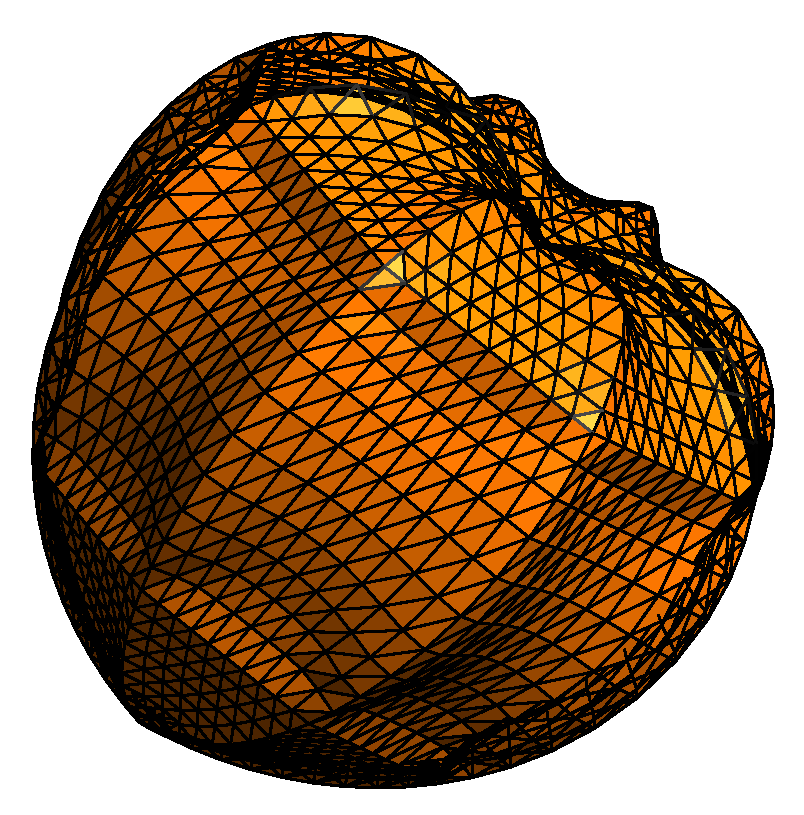
\includegraphics[width=70mm]{fisalis-round}
  \caption{Not yet a physalis}
  \label{\numb section 2.\numb fig 13}
\end{figure}

This shape is still not satisfactory, so we apply a deformation in $ \mathbb{R}^3 $ in order to
get a sharper tip.
The {\small\tt apple} manifold is no longer relevant.

\begin{Verbatim}[commandchars=\\\{\},formatcom=\small\tt,frame=single,
   label=parag-\ref{\numb section 2.\numb parag 11}.cpp,rulecolor=\color{coment},
   baselinestretch=0.94,framesep=2mm]
   \verm{CellIterator} \azul{it} = fisalis.iterator ( \verm{tag}::over_vertices );
   for ( it.reset(); it.in_range(); it++ )
   \{  \verm{Cell} \azul{P} = *it;
      x(P) *= 0.8;  y(P) *= 0.8;
      if ( z(P) > 1.3 )
      \{	 x(P) = x(P) / ( 1. + 300. * std::pow ( z(P) - 1.3, 3. ) );
         y(P) = y(P) / ( 1. + 300. * std::pow ( z(P) - 1.3, 3. ) );
         z(P) = z(P) * ( 1. + 10. * ( z(P) - 1.3 ) * ( z(P) - 1.3 ) );  \}
      if ( z(P) > 0. ) z(P) *= 0.8;                                        \}
\end{Verbatim}

Paragraph \ref{\numb section 9.\numb parag 3} explains the notion of an iterator over cells.

We add a sequence of baricenter operations for smoothening the shape.
Note that each baricenter operation is relative to a sector and it applies only to inner
vertices, so the boundary of the sector is not changed.
Thus, the eight rims defined in the beginning are kept unchanged.

\begin{Verbatim}[commandchars=\\\{\},formatcom=\small\tt,frame=single,
   label=parag-\ref{\numb section 2.\numb parag 11}.cpp,rulecolor=\color{coment},
   baselinestretch=0.94,framesep=2mm]
   std::list<\verm{Mesh}>::iterator \azul{it1};
   for ( it1 = lm.begin(); it1 != lm.end(); it1++ )
   \{  \verm{Mesh} \azul{sect} = *it1;
      \verm{CellIterator} \azul{it2} = sect.iterator ( \verm{tag}::over_vertices );
      for ( int \azul{i} = 1; i < 20; i++ )
      for ( it2.reset(); it2.in_range(); it2++ )
      \{  \verm{Cell} \azul{ver} = *it2;
         if ( ver.is_inner_to ( sect ) ) sect.baricenter ( ver );  \}                     \}
\end{Verbatim}

And we are happy with the final result, shown in figure \ref{\numb section 2.\numb fig 14}.

\begin{figure}[ht] \centering
  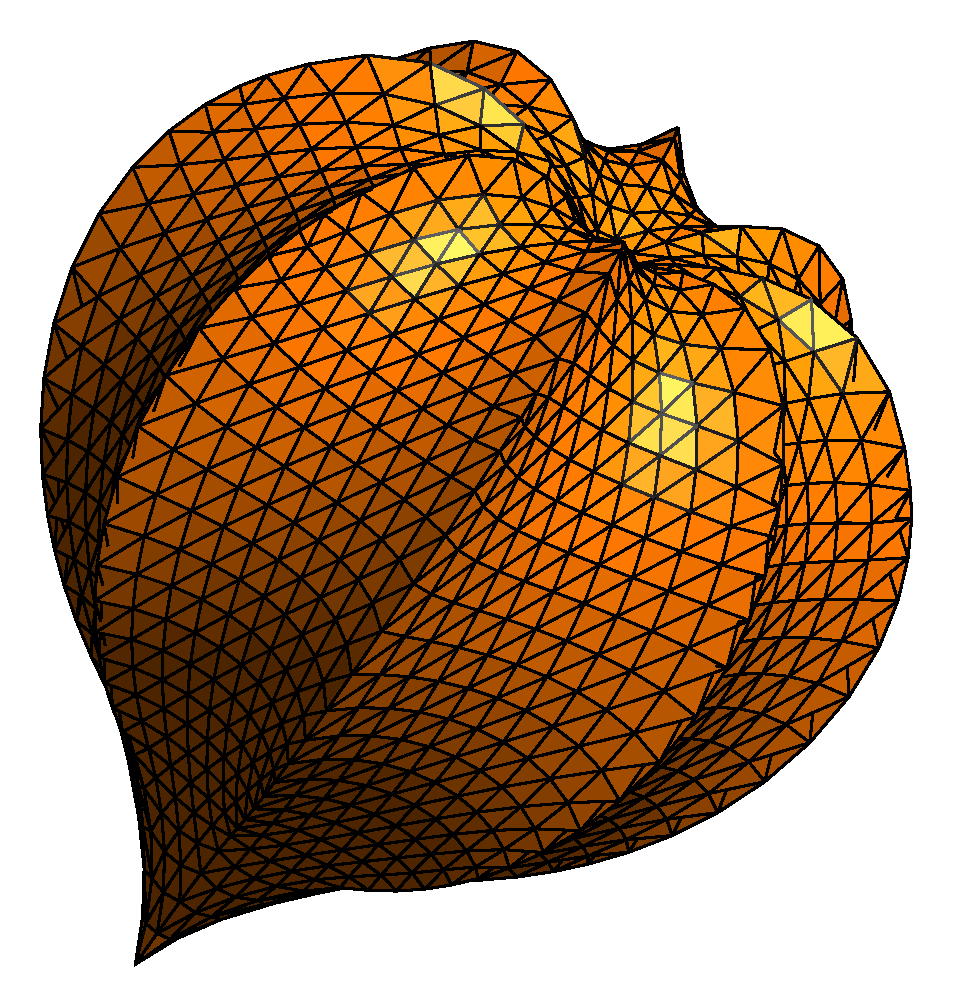
\includegraphics[width=75mm]{fisalis}
  \caption{Meshing a chinese lantern}
  \label{\numb section 2.\numb fig 14}
\end{figure}

An animation related to this example is available at\hfil\break
{\small\tt http://manifem.rd.ciencias.ulisboa.pt/apple-to-physalis.gif}


          %-----------------------------------%
\section{~~A manifold defined by two equations}\label{\numb section 2.\numb parag 12}
          %-----------------------------------%

We can define a one-dimensional submanifold of $ \mathbb{R}^3 $ by two implicit equations :
\medskip

\begin{figure}[ht] \centering
  \psfrag{S}{\tt\textcolor{textindraw}{S}}
  \psfrag{N}{\tt\textcolor{textindraw}{N}}
  \psfrag{E}{\tt\textcolor{textindraw}{E}}
  \psfrag{W}{\tt\textcolor{textindraw}{W}}
  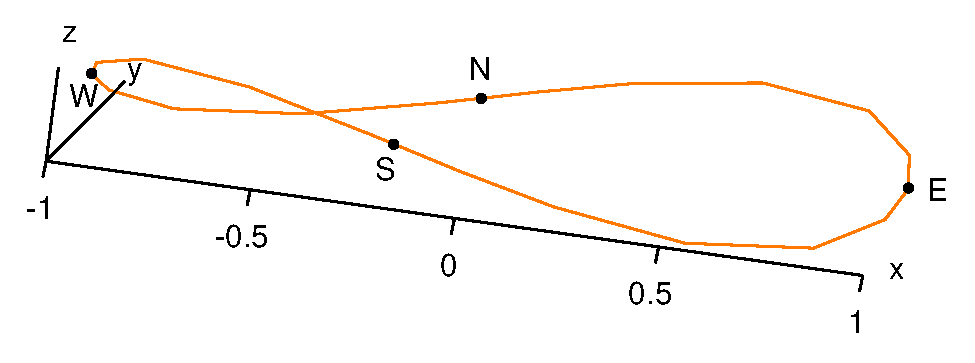
\includegraphics[width=95mm]{circle-3d}
  \caption{One-dimensional mesh in $ {\mathbb R}^3 $}
  \label{\numb section 2.\numb fig 15}
\end{figure}

\begin{Verbatim}[commandchars=\\\{\},formatcom=\small\tt,frame=single,
   label=parag-\ref{\numb section 2.\numb parag 12}.cpp,rulecolor=\color{coment},
   baselinestretch=0.94,framesep=2mm]
   \verm{Manifold} \azul{RR3} ( \verm{tag}::Euclid, \verm{tag}::of_dim, 3 );
   \verm{Function} \azul{xyz} = RR3.build_coordinate_system ( \verm{tag}::Lagrange, \verm{tag}::of_degree, 1 );
   \verm{Function} \azul{x} = xyz[0],  \azul{y} = xyz[1],  \azul{z} = xyz[2];

   \verm{Manifold} \azul{circle_manifold} = RR3.implicit ( x*x + y*y == 1., x*y == 4.*z );
   \verm{Cell} \azul{S} ( \verm{tag}::vertex );  x(S) =  0.;   y(S) = -1.;  z(S) = 0.;
   \verm{Cell} \azul{E} ( \verm{tag}::vertex );  x(E) =  1.;   y(E) =  0.;  z(E) = 0.;
   \verm{Cell} \azul{N} ( \verm{tag}::vertex );  x(N) =  0.;   y(N) =  1.;  z(N) = 0.;
   \verm{Cell} \azul{W} ( \verm{tag}::vertex );  x(W) = -1.;   y(W) =  0.;  z(W) = 0.;
   \cinza{// these four points already belong to 'circle_manifold', no projection needed}
   \verm{Mesh} \azul{SE} ( \verm{tag}::segment, S.reverse(), E, \verm{tag}::divided_in, 5 );
   \verm{Mesh} \azul{EN} ( \verm{tag}::segment, E.reverse(), N, \verm{tag}::divided_in, 5 );
   \verm{Mesh} \azul{NW} ( \verm{tag}::segment, N.reverse(), W, \verm{tag}::divided_in, 5 );
   \verm{Mesh} \azul{WS} ( \verm{tag}::segment, W.reverse(), S, \verm{tag}::divided_in, 5 );
   \verm{Mesh} \azul{circle} ( \verm{tag}::join, SE, EN, NW, WS );
\end{Verbatim}

Paragraph \ref{\numb section 3.\numb parag 4} shows another way of meshing the same loop.


          %------------------------------%
\section{~~A submanifold of a submanifold}\label{\numb section 2.\numb parag 13}
          %------------------------------%

An implicit manifold has submanifolds.
For instance, we can improve the look of the ``bumpy hemisphere'' in paragraph
\ref{\numb section 2.\numb parag 7} by building its base (a circle-like closed curve)
inside a one-dimensional manifold.
For the rest of the surface, we switch back to the two-dimensional manifold {\small\tt nut} :
\medskip

\begin{figure}[ht] \centering
  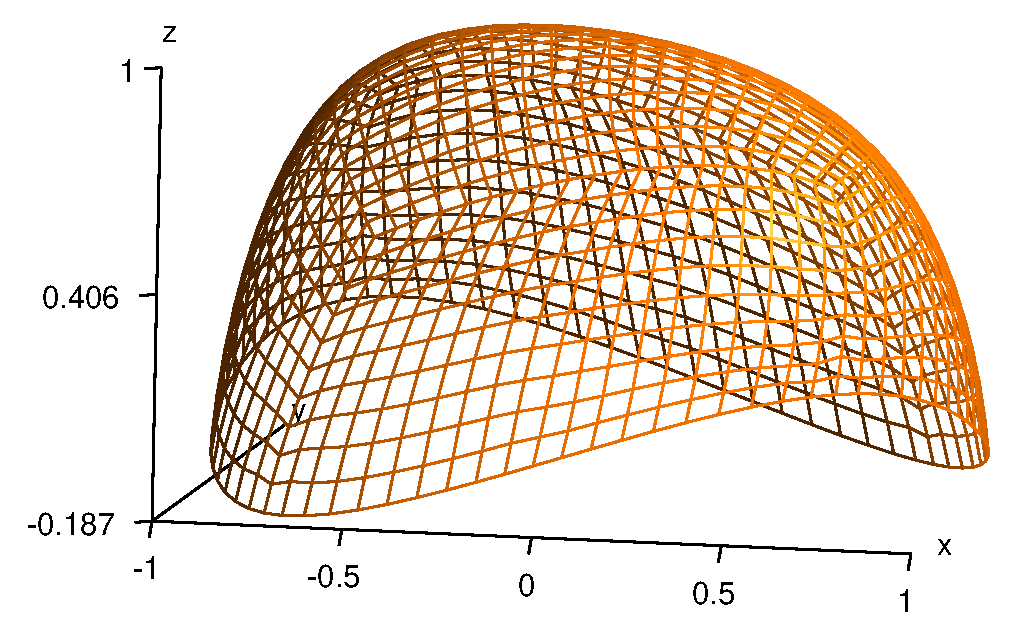
\includegraphics[width=105mm]{bumpy}
  \caption{A shell}
  \label{\numb section 2.\numb fig 16}
\end{figure}

\begin{Verbatim}[commandchars=\\\{\},formatcom=\small\tt,frame=single,
   label=parag-\ref{\numb section 2.\numb parag 13}.cpp,rulecolor=\color{coment},
   baselinestretch=0.94,framesep=2mm]
   \verm{Manifold} \azul{nut} = RR3.implicit ( x*x + y*y + z*z + 1.5*x*y*z == 1. );
   int \azul{n} = 10;

   \cinza{// first build the base (a closed curve)}
   \verm{Manifold} \azul{base} = nut.implicit ( x*x + 3.*z == 0. );

   \verm{Cell} \azul{S} ( \verm{tag}::vertex );    x(S)  =   0.;   y(S)  =  -1.;   z(S)  =  0.;
   \verm{Cell} \azul{E} ( \verm{tag}::vertex );    x(E)  =   1.;   y(E)  =   0.;   z(E)  =  0.;
   \verm{Cell} \azul{N} ( \verm{tag}::vertex );    x(N)  =   0.;   y(N)  =   1.;   z(N)  =  0.;
   \verm{Cell} \azul{W} ( \verm{tag}::vertex );    x(W)  =  -1.;   y(W)  =   0.;   z(W)  =  0.;
   \cinza{// no need to project S and N, they are already on 'base'}
   base.project(E);  base.project(W);
   \verm{Cell} \azul{mSW} ( \verm{tag}::vertex );  x(mSW) = -1.;   y(mSW) = -1.;   z(mSW) = 0.;
   base.project ( mSW );  \cinza{// midway between S and W}
   \verm{Cell} \azul{mSE} ( \verm{tag}::vertex );  x(mSE) =  1.;   y(mSE) = -1.;   z(mSW) = 0.;
   base.project ( mSE );  \cinza{// midway between S and E}
   \cinza{// define similarly mNE and mNW}

   \cinza{// now build eight segments, forming the base}
   \verm{Mesh} \azul{S_mSW} ( \verm{tag}::segment, S.reverse(), mSW, \verm{tag}::divided_in, n );
   \verm{Mesh} \azul{S_mSE} ( \verm{tag}::segment, S.reverse(), mSE, \verm{tag}::divided_in, n );
   \verm{Mesh} \azul{E_mSE} ( \verm{tag}::segment, E.reverse(), mSE, \verm{tag}::divided_in, n );
   \verm{Mesh} \azul{E_mNE} ( \verm{tag}::segment, E.reverse(), mNE, \verm{tag}::divided_in, n );
   \verm{Mesh} \azul{N_mNE} ( \verm{tag}::segment, N.reverse(), mNE, \verm{tag}::divided_in, n );
   \verm{Mesh} \azul{N_mNW} ( \verm{tag}::segment, N.reverse(), mNW, \verm{tag}::divided_in, n );
   \verm{Mesh} \azul{W_mSW} ( \verm{tag}::segment, W.reverse(), mSW, \verm{tag}::divided_in, n );
   \verm{Mesh} \azul{W_mNW} ( \verm{tag}::segment, W.reverse(), mNW, \verm{tag}::divided_in, n );

   \cinza{// we are done with the base, now switch back to 'nut'}
   nut.set_as_working_manifold();
   \cinza{// more points :}
   \verm{Cell} \azul{up} ( \verm{tag}::vertex );   x(up) =   0.;   y(up) =   0.;   z(up) =  1.;
   \cinza{// no need to project 'up', it is already on 'nut'}
   \verm{Cell} \azul{mSup}  ( \verm{tag}::vertex );  x(mSup) =  0.;   y(mSup) = -1.;   z(mSup) = 1.;
   nut.project ( mSup );  \cinza{// midway between S and up}
   \verm{Cell} \azul{mSWup} ( \verm{tag}::vertex );  x(mSWup) = -1.;  y(mSWup) = -1.;  z(mSWup) = 1.;
   nut.project ( mSWup );  \cinza{// somewhere between S, W and up}
   \cinza{// ... and so forth ...}

   \cinza{// more segments :}
   \verm{Mesh} \azul{W_mWup} ( \verm{tag}::segment, W.reverse(), mWup, \verm{tag}::divided_in, n );
   \verm{Mesh} \azul{mSW_mSWup} ( \verm{tag}::segment, mSW.reverse(), mSWup, \verm{tag}::divided_in, n );
   \verm{Mesh} \azul{mWup_mSWup} ( \verm{tag}::segment, mWup.reverse(), mSWup, \verm{tag}::divided_in, n );
   \cinza{// ... and so forth ...}
\end{Verbatim}

If we wanted a flat base, we could have defined

\begin{Verbatim}[commandchars=\\\{\},formatcom=\small\tt,baselinestretch=0.94]
   \verm{Manifold} \azul{base} = nut.implicit ( z == 0. );
\end{Verbatim}

Paragraph \ref{\numb section 3.\numb parag 9} shows a way to mesh the same surface using
fewer lines of code.


          %-------------------------------%
\section{~~Parametric manifolds -- a curve}\label{\numb section 2.\numb parag 14}
          %-------------------------------%

Paragraphs \ref{\numb section 2.\numb parag 4} -- \ref{\numb section 2.\numb parag 13} describe
manifolds defined through implicit equations, that is, level sets in $ \mathbb{R}^2 $ or
$ \mathbb{R}^3 $.
Another way of defining a submanifold is through a parametrization.
Below is an example.

\begin{figure}[ht] \centering
  \psfrag{A}{\tt\textcolor{textindraw}{A}}
  \psfrag{B}{\tt\textcolor{textindraw}{B}}
  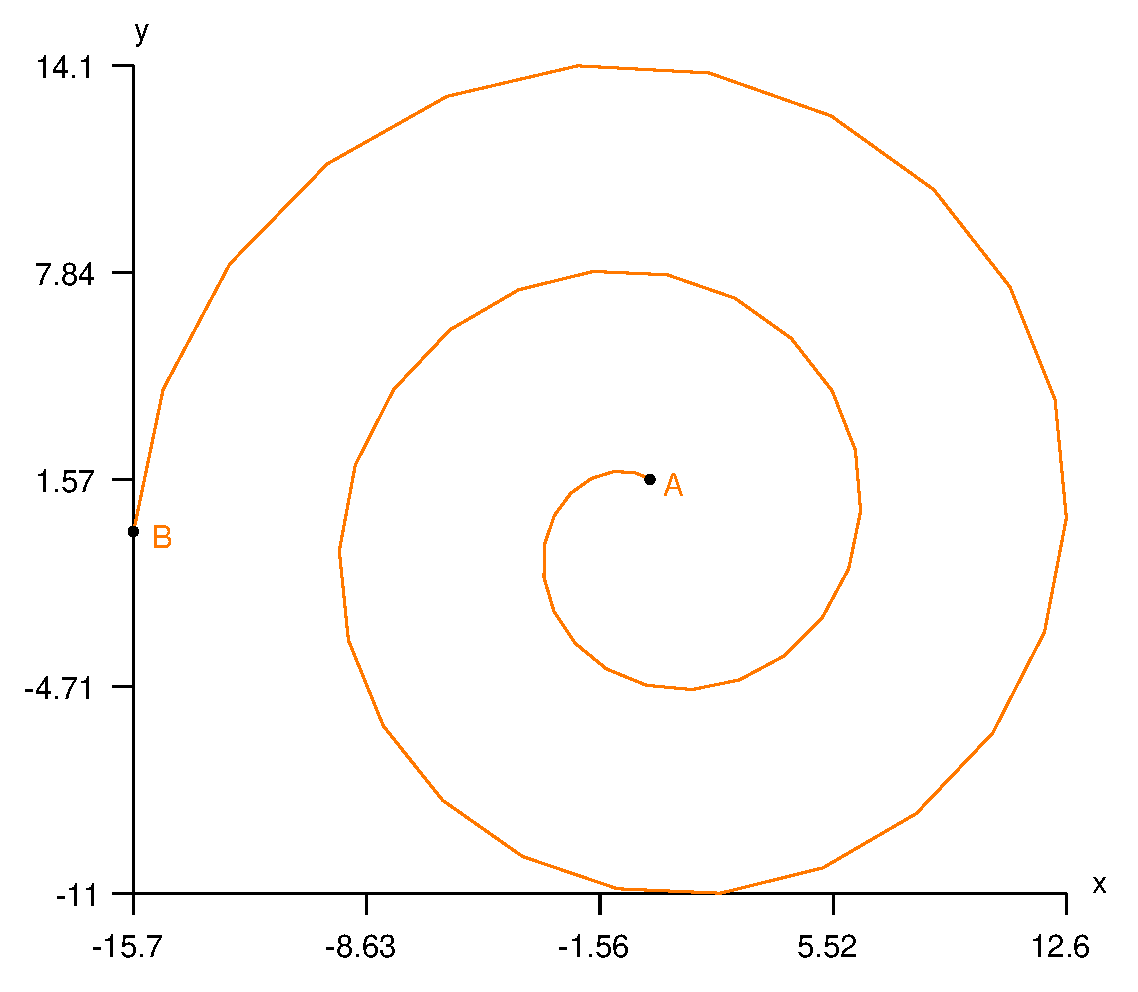
\includegraphics[width=65mm]{spiral}
  \caption{One-dimensional mesh in $ {\mathbb R}^2 $}
\end{figure}

\begin{Verbatim}[commandchars=\\\{\},formatcom=\small\tt,frame=single,
   label=parag-\ref{\numb section 2.\numb parag 14}.cpp,rulecolor=\color{coment},
   baselinestretch=0.94,framesep=2mm]
   \cinza{// at the beginning, we define 'spiral' as a straight line}
   \verm{Manifold} \azul{spiral} ( \verm{tag}::Euclid, \verm{tag}::of_dim, 1 );
   \verm{Function} \azul{t} = spiral.build_coordinate_system ( \verm{tag}::Lagrange, \verm{tag}::of_degree, 1 );

   \cinza{// now build 'arc_of_spiral' merely as a segment from pi/2 to 5 pi}
   const double \azul{pi} = 3.1415926536;
   \verm{Cell} \azul{A} ( \verm{tag}::vertex );  t(A) =  pi/2.;
   \verm{Cell} \azul{B} ( \verm{tag}::vertex );  t(B) =  5.*pi;
   \verm{Mesh} \azul{arc_of_spiral} ( \verm{tag}::segment, A.reverse(), B, \verm{tag}::divided_in, 30 );
   \cinza{// not very interesting for now}
   \cinza{// but now define functions x and y as expressions of t :}
   \verm{Function} \azul{x} = t*\verm{cos}(t), \azul{y} = t*\verm{sin}(t);
   \cinza{// and declare them to be the new coordinates on the 'spiral' manifold}
   spiral.set_coordinates ( x && y );

   \cinza{// in future statements (e.g. for graphical representation)}
   \cinza{// x and y will be used, not t :}
   arc_of_spiral.draw_ps (\verde{"spiral.eps"});
\end{Verbatim}

The operator {\small\tt \&\&} joins two functions into one vector function.

Note that, when defining points {\small\tt A} and {\small\tt B}, we only set the value of {\small\tt t}.
Functions {\small\tt x} and {\small\tt y} are defined later, as arithmetic expressions in terms of
{\small\tt t}; their values will be computed ``on-the-fly'' when needed.
%A parametric manifold has attached to it a function called ``parameter'' and another one called
%``coordinate''.
%Both may be vector functions (may have serveral components).
%The ``coordinates'' are used, for instance, for graphical representation.
%The ``parameter'' or ``parameters'' are used, for instance, for interpolation.
%The {\small\tt \verm{Mesh}} constructors with {\small\tt \verm{tag}::segment}, {\small\tt \verm{tag}::quadrangle} or
%{\small\tt \verm{tag}::triangle} build new points and define their position in the manifold by
%interpolating the parameters, not the coordinates.
%Unlike for implicit manifolds, no projection is necessary.
In the drawing above, we note that the generated points are not equidistant in the sense of the
Euclidian distance in $ \mathbb{R}^2 $.
They correspond to values of {\small\tt t} which are uniformly distributed between
$ \pi/2 $ (at {\small\tt A}) and $ 5\pi $ (at {\small\tt B}).

The approach described above has the disadvantage that, if we want to subsequently change the
distribution of nodes along the {\small\tt arc\_\,of\_\,spiral}, we must switch back to the original
{\small\tt t} coordinate.

Paragraph \ref{\numb section 3.\numb parag 5} shows another way of meshing a curve,
producing equidistant vertices.


          %----------------%
\section{~~Closing a circle}\label{\numb section 2.\numb parag 15}
          %----------------%

In the approach of paragraph \ref{\numb section 2.\numb parag 14}, it is possible but cumbersome to
build a closed curve :

\begin{Verbatim}[commandchars=\\\{\},formatcom=\small\tt,frame=single,
   label=parag-\ref{\numb section 2.\numb parag 15}.cpp,rulecolor=\color{coment},
   baselinestretch=0.94,framesep=2mm]
   \verm{Manifold} \azul{circle_manif} ( \verm{tag}::Euclid, \verm{tag}::of_dim, 1 );
   \verm{Function} \azul{t} = circle_manif.build_coordinate_system
      ( \verm{tag}::Lagrange, \verm{tag}::of_degree, 1 );

   \cinza{// build 'circle' merely as a segment from 0 to 1.9 pi}
   const double \azul{pi} = 3.1415926536;
   \verm{Cell} \azul{A} ( \verm{tag}::vertex );  t(A) =  0.;
   \verm{Cell} \azul{B} ( \verm{tag}::vertex );  t(B) =  1.9*pi;
   \verm{Mesh} \azul{circle} ( \verm{tag}::segment, A.reverse(), B, \verm{tag}::divided_in, 19 );

   \cinza{// now close the curve in a not very elegant manner}
   \verm{Cell} \azul{BA} ( \verm{tag}::segment, B.reverse(), A );
   BA.add_to ( circle );

   \cinza{// define new coordinates on circle_manif as expressions of t :}
   \verm{Function} \azul{x} = \verm{cos}(t), \azul{y} = \verm{sin}(t);
   circle_manif.set_coordinates ( x && y );

   \cinza{// in future statements (e.g. for graphical representation)}
   \cinza{// x and y will be used, not t :}
   circle.draw_ps (\verde{"circle.eps"});
\end{Verbatim}

% When we build a segment {\small\tt \verm{Cell}} like {\small\tt BA} above, we must provide a negative vertex
% (the base of the segment) and a positive one (the tip of the segment).
% That is why we give {\small\tt B.reverse()} as argument rather than {\small\tt B}.
% This is quite different from building a segment {\small\tt \verm{Mesh}}, when we provide two positive
% vertices as arguments, along with the number of divisions.

Paragraph \ref{\numb section 7.\numb parag 2} shows a more elegant way to close a curve in itself.

On the other hand, if we only want a visual illusion of a closed circle, we may use the code below.

\begin{Verbatim}[commandchars=\\\{\},formatcom=\small\tt,baselinestretch=0.94]
   \verm{Manifold} \azul{circle_manif} ( \verm{tag}::Euclid, \verm{tag}::of_dim, 1 );
   \verm{Function} \azul{t} = circle_manif.build_coordinate_system
      ( \verm{tag}::Lagrange, \verm{tag}::of_degree, 1 );

   \cinza{// build 'circle' merely as a segment from 0 to 2 pi}
   const double \azul{pi} = 3.1415926536;
   \verm{Cell} \azul{A} ( \verm{tag}::vertex );  t(A) =  0.;
   \verm{Cell} \azul{B} ( \verm{tag}::vertex );  t(B) =  2.*pi;
   \verm{Mesh} \azul{circle} ( \verm{tag}::segment, A.reverse(), B, \verm{tag}::divided_in, 20 );
   \cinza{// gives the illusion of a closed circle}

   \cinza{// define new coordinates on circle_manif as expressions of t :}
   \verm{Function} \azul{x} = \verm{cos}(t), \azul{y} = \verm{sin}(t);
   circle_manif.set_coordinates ( x && y );
\end{Verbatim}


          %---------------------------------%
\section{~~Parametric manifolds -- a surface}\label{\numb section 2.\numb parag 16}
          %---------------------------------%

Here is an example of a parametrized surface :

\begin{figure}[ht] \centering
  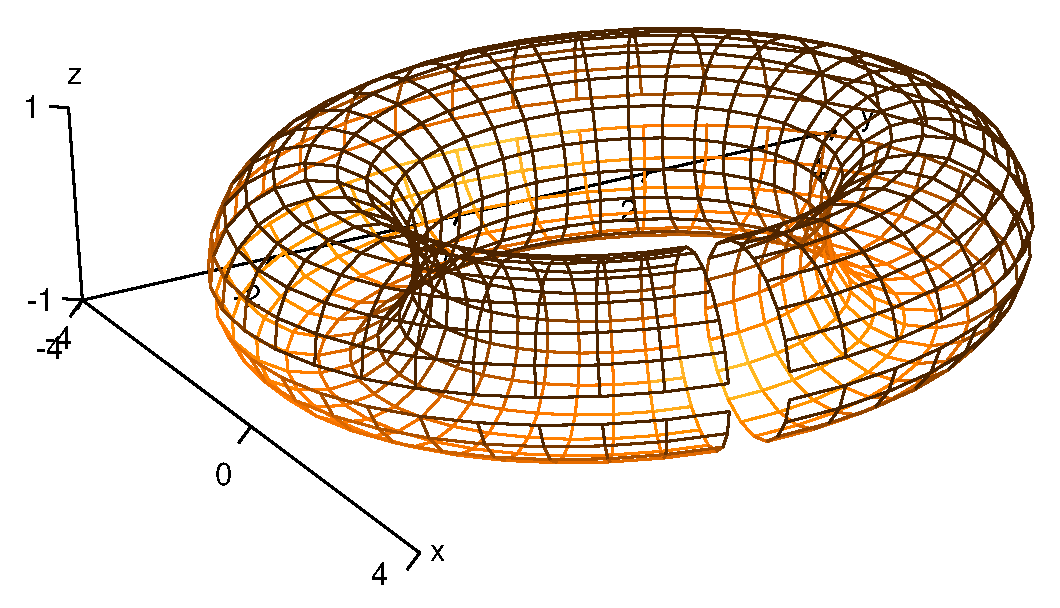
\includegraphics[width=125mm]{torus}
  \caption{Incomplete torus}
\end{figure}

\begin{Verbatim}[commandchars=\\\{\},formatcom=\small\tt,frame=single,
   label=parag-\ref{\numb section 2.\numb parag 16}.cpp,rulecolor=\color{coment},
   baselinestretch=0.94,framesep=2mm]
   \verm{Manifold} \azul{torus} ( \verm{tag}::Euclid, \verm{tag}::of_dim, 2 );
   \verm{Function} \azul{alpha_beta} =
      torus.build_coordinate_system ( \verm{tag}::Lagrange, \verm{tag}::of_degree, 1 );

   \cinza{// extract components of alpha_beta :}
   \verm{Function} \azul{alpha} = alpha_beta[0], \azul{beta} = alpha_beta[1];
   \cinza{// build a rectangle in the alpha-beta plane}
   const double \azul{pi} = 3.1415926536;
   \verm{Cell} \azul{A} ( \verm{tag}::vertex );  alpha(A) = 0.;       beta(A) = 0.;
   \verm{Cell} \azul{B} ( \verm{tag}::vertex );  alpha(B) = 0.;       beta(B) = 1.9*pi;
   \verm{Cell} \azul{C} ( \verm{tag}::vertex );  alpha(C) = 1.95*pi;  beta(C) = 1.9*pi;
   \verm{Cell} \azul{D} ( \verm{tag}::vertex );  alpha(D) = 1.95*pi;  beta(D) = 0.;

   \cinza{// four almost-closed circles :}
   \verm{Mesh} \azul{AB} ( \verm{tag}::segment, A.reverse(), B, \verm{tag}::divided_in, 19 );
   \verm{Mesh} \azul{BC} ( \verm{tag}::segment, B.reverse(), C, \verm{tag}::divided_in, 39 );
   \verm{Mesh} \azul{CD} ( \verm{tag}::segment, C.reverse(), D, \verm{tag}::divided_in, 19 );
   \verm{Mesh} \azul{DA} ( \verm{tag}::segment, D.reverse(), A, \verm{tag}::divided_in, 39 );
   \verm{Mesh} \azul{ABCD} ( \verm{tag}::rectangle, AB, BC, CD, DA );  \cinza{// an almost-closed torus}
   \cinza{// parametrize the torus}
   const double \azul{big_radius} = 3., \azul{small_radius} = 1.;
   \verm{Function} \azul{x} = ( big_radius + small_radius * \verm{cos}(beta) ) * \verm{cos}(alpha),
            \azul{y} = ( big_radius + small_radius * \verm{cos}(beta) ) * \verm{sin}(alpha),
            \azul{z} = small_radius * \verm{sin}(beta);

   torus.set_coordinates ( x && y && z );  \cinza{// forget about alpha and beta}
   \cinza{// in future statements (e.g. for graphical representation)}
   \cinza{// x, y and z will be used, not alpha nor beta :}
   ABCD.export_msh (\verde{"torus.msh"});
\end{Verbatim}

Closing the torus in the cumbersome manner shown in paragraph
\ref{\numb section 2.\numb parag 15} is possible but not practical.
Paragraph \ref{\numb section 7.\numb parag 5} shows a more elegant solution.

If we only want a visual illusion of a closed surface, we may use the code below

\begin{Verbatim}[commandchars=\\\{\},formatcom=\small\tt,baselinestretch=0.94]
   \verm{Cell} \azul{A} ( \verm{tag}::vertex );  alpha(A) = 0.;     beta(A) = 0.;
   \verm{Cell} \azul{B} ( \verm{tag}::vertex );  alpha(B) = 0.;     beta(B) = 2.*pi;
   \verm{Cell} \azul{C} ( \verm{tag}::vertex );  alpha(C) = 2.*pi;  beta(C) = 2.*pi;
   \verm{Cell} \azul{D} ( \verm{tag}::vertex );  alpha(D) = 2.*pi;  beta(D) = 0.;
   \verm{Mesh} \azul{AB} ( \verm{tag}::segment, A.reverse(), B, \verm{tag}::divided_in, 20 );
   \verm{Mesh} \azul{BC} ( \verm{tag}::segment, B.reverse(), C, \verm{tag}::divided_in, 40 );
   \verm{Mesh} \azul{CD} ( \verm{tag}::segment, C.reverse(), D, \verm{tag}::divided_in, 20 );
   \verm{Mesh} \azul{DA} ( \verm{tag}::segment, D.reverse(), A, \verm{tag}::divided_in, 40 );
   \cinza{// AB, BC, CD and DA look like closed circles}
   \verm{Mesh} \azul{ABCD} ( \verm{tag}::rectangle, AB, BC, CD, DA );
   \cinza{// ABCD gives the illusion of a closed torus}
\end{Verbatim}


          %-----------------------------------------%
\section{~~Starting with a high-dimensional manifold}\label{\numb section 2.\numb parag 17}
          %-----------------------------------------%

Instead of starting with a manifold having only the parameter(s), we may start with a
high-dimensional manifold containing both the geometric coordinates and the parameter(s),
then define the parametrization through equation(s).
% The advantage of this approach is that we can later shwitch on and off a constraint,
% thus switching between meshes of different dimensions.
There is a disadvantage however, regarding performance : {\maniFEM} will reserve,
for each vertex, space in the computer's memory for five {\small\tt double} values.

\begin{Verbatim}[commandchars=\\\{\},formatcom=\small\tt,frame=single,
   label=parag-\ref{\numb section 2.\numb parag 17}.cpp,rulecolor=\color{coment},
   baselinestretch=0.94,framesep=2mm]
   \verm{Manifold} \azul{RR5} ( \verm{tag}::Euclid, \verm{tag}::of_dim, 5 );
   \verm{Function} \azul{xyzab} = RR5.build_coordinate_system ( \verm{tag}::Lagrange, \verm{tag}::of_degree, 1 );
   \cinza{// extract components of xyzab :}
   \verm{Function} \azul{x} = xyzab[0], \azul{y} = xyzab[1], \azul{z} = xyzab[2],
                   \azul{alpha} = xyzab[3], \azul{beta} = xyzab[4];
   \cinza{// define a torus as a submanifold of RR5 :}
   const double \azul{big_radius} = 3, \azul{small_radius} = 1;
   \verm{Manifold} \azul{torus} = RR5.parametric
      ( x == ( big_radius + small_radius * \verm{cos}(beta) ) * \verm{cos}(alpha),
        y == ( big_radius + small_radius * \verm{cos}(beta) ) * \verm{sin}(alpha),
        z == small_radius * \verm{sin}(beta)                                );
   const double \azul{pi} = 3.1415926536;
        
   \cinza{// define four corners :}
   \verm{Cell} \azul{A} ( \verm{tag}::vertex );  alpha(A) = 0.;      beta(A) = 0.;      torus.project(A);
   \verm{Cell} \azul{B} ( \verm{tag}::vertex );  alpha(B) = 0.;      beta(B) = 1.9*pi;  torus.project(B);
   \verm{Cell} \azul{C} ( \verm{tag}::vertex );  alpha(C) = 1.95*pi; beta(C) = 1.9*pi;  torus.project(C);
   \verm{Cell} \azul{D} ( \verm{tag}::vertex );  alpha(D) = 1.95*pi; beta(D) = 0.;      torus.project(D);
   \cinza{// four almost-closed circles :}
   \verm{Mesh} \azul{AB} ( \verm{tag}::segment, A.reverse(), B, \verm{tag}::divided_in, 19 );
   \verm{Mesh} \azul{BC} ( \verm{tag}::segment, B.reverse(), C, \verm{tag}::divided_in, 39 );
   \verm{Mesh} \azul{CD} ( \verm{tag}::segment, C.reverse(), D, \verm{tag}::divided_in, 19 );
   \verm{Mesh} \azul{DA} ( \verm{tag}::segment, D.reverse(), A, \verm{tag}::divided_in, 39 );

   \cinza{// build a rectangle}
   \verm{Mesh} \azul{ABCD} ( \verm{tag}::rectangle, AB, BC, CD, DA );  \cinza{// an almost-closed torus}

   \cinza{// forget about alpha and beta :}
   torus.set_coordinates ( x && y && z );

   \cinza{// in future statements (e.g. for graphical representation)}
   \cinza{// x, y and z will be used, not alpha nor beta :}
   ABCD.export_msh (\verde{"torus.msh"});
\end{Verbatim}

The {\small\tt \verm{Manifold}::parametric} method is similar to {\small\tt \verm{Manifold}::implicit},
presented in paragraphs \ref{\numb section 2.\numb parag 4} --
\ref{\numb section 2.\numb parag 13}.
The only difference is that by using {\small\tt parametric} we declare an explicit dependence%
\footnote {Perhaps {\small\tt explicit} would be a better name than {\small\tt parametric};
unfortunately, that word is reserved in {\small\tt C++}.}
of the coordinates (here, {\small\tt x}, {\small\tt y} and {\small\tt z}) upon the parameters
(here, {\small\tt alpha} and {\small\tt beta}).
This endows the manifold {\small\tt torus} with a different projection operator.
The projection of a vertex from {\small\tt RR5} onto {\small\tt torus} is done by merely updating
the values of {\small\tt x}, {\small\tt y} and {\small\tt z}, while keeping {\small\tt alpha} and
{\small\tt beta} constant.
